\documentclass[lettersize,journal]{IEEEtran}
\IEEEoverridecommandlockouts

\usepackage{cite}
\usepackage{amsmath,amssymb,amsfonts}
\usepackage{graphicx}
\usepackage{textcomp}
\usepackage{xcolor}
\usepackage{booktabs}
\usepackage{multirow}
\usepackage{float}
\usepackage{algorithm}
\usepackage{algorithmic}
\usepackage{url}
\usepackage{stfloats}
\usepackage{enumitem}

\setlist{nosep,leftmargin=*}

\setlength{\textfloatsep}{8pt plus 2pt minus 2pt}
\setlength{\dbltextfloatsep}{8pt plus 2pt minus 2pt}
\setlength{\floatsep}{6pt plus 2pt minus 2pt}
\setlength{\intextsep}{6pt plus 2pt minus 2pt}
\setlength{\abovedisplayskip}{6pt plus 2pt minus 2pt}
\setlength{\belowdisplayskip}{6pt plus 2pt minus 2pt}
\setlength{\abovedisplayshortskip}{4pt plus 2pt minus 2pt}
\setlength{\belowdisplayshortskip}{4pt plus 2pt minus 2pt}
% Fill pages more tightly around floats (fewer half-empty float pages)
\renewcommand{\topfraction}{0.95}
\renewcommand{\bottomfraction}{0.95}
\renewcommand{\textfraction}{0.05}
\renewcommand{\floatpagefraction}{0.85}
\renewcommand{\dbltopfraction}{0.95}
\renewcommand{\dblfloatpagefraction}{0.85}
\setcounter{topnumber}{3}
\setcounter{bottomnumber}{3}
\setcounter{totalnumber}{6}
\setcounter{dbltopnumber}{3}
% Reduce vertical spacing around section headings (IEEEtran journal default is large)
\makeatletter
\renewcommand{\section}{\@startsection{section}{1}{\z@}{1.5ex plus 1ex minus 0.5ex}{0.7ex plus 1ex minus 0ex}{\normalfont\normalsize\centering\scshape}}
\renewcommand{\subsection}{\@startsection{subsection}{2}{\z@}{2.0ex plus 1ex minus 0.5ex}{0.7ex plus .5ex minus 0ex}{\normalfont\normalsize\itshape}}
\makeatother

\def\BibTeX{{\rm B\kern-.05em{\sc i\kern-.025em b}\kern-.08em
    T\kern-.1667em\lower.7ex\hbox{E}\kern-.125emX}}

\begin{document}

\title{Progressive Digital Semantic Speech Communication for Packet-Loss Channels}

\author{Hao~Cheng,~\IEEEmembership{Student~Member,~IEEE,}
        Wei~Chen,~\IEEEmembership{Member,~IEEE,}
        Bo~Ai,~\IEEEmembership{Fellow,~IEEE,}
        Xiongkuo~Min,~\IEEEmembership{Member,~IEEE,}
        Guangtao~Zhai,~\IEEEmembership{Senior~Member,~IEEE,} and
        Wenwu~Wang,~\IEEEmembership{Fellow,~IEEE}%
\thanks{H. Cheng, W. Chen, and B. Ai are with the School of Electronic and Information Engineering, Beijing Jiaotong University, Beijing 100044, China (e-mail: \{24125150, weich, boai\}@bjtu.edu.cn).}%
\thanks{X. Min and G. Zhai are with the Institute of Image Communication and Network Engineering, Department of Electronic Engineering, Shanghai Jiao Tong University, Shanghai 200240, China (e-mail: \{minxiongkuo, zhaiguangtao\}@sjtu.edu.cn).}%
\thanks{W. Wang is with the School of Computer Science and Electronic Engineering, University of Surrey, Guildford GU2 7XH, U.K., and also with the Surrey Institute for People Centred AI (e-mail: W.Wang@surrey.ac.uk).}%
\thanks{Manuscript received Month xx, 2026; revised Month xx, 2026.}%
\thanks{Corresponding author: Bo Ai.}}

% The paper headers
\markboth{IEEE TRANSACTIONS ON WIRELESS COMMUNICATIONS,~Vol.~XX, No.~XX, Month~2026}%
{Cheng \MakeLowercase{\textit{et al.}}: Progressive Digital Semantic Speech Communication for Packet-Loss Channels}

\maketitle

\begin{abstract}
Non-terrestrial networks (NTNs), together with their integration with terrestrial infrastructure, support speech services in remote, offshore, moving-platform, and emergency-response scenarios, where bandwidth is scarce, packet loss is prevalent, and real-time operation is required. In this regime, conventional speech codecs become inefficient at low bitrates, while existing speech semantic communication methods still struggle to combine low-bitrate transmission, packet-loss robustness, and low-latency deployment within one framework. To address this, we propose Progressive Digital Semantic Speech Communication (PDSSC), which uses a semantic-priority layered discrete representation, with the lowest layers carrying semantic content and speaker timbre and progressively finer acoustic detail above, enabling progressive transmission at low bitrates. For stable user populations, our method treats bitrate reduction and packet loss as a speaker-related recovery problem, addressed by a low-step generative recovery model leveraging same-speaker reference side information from a receiver-maintained library. A lightweight bitrate controller is also introduced for flexible deployment. Experimental results on LibriSpeech show that the proposed method achieves better perceptual quality than Opus while reducing transmission bitrate by 87.5\%, and exhibits stronger robustness under packet-loss conditions, with a complexity and latency analysis further confirming its practicality for real-time deployment.
\end{abstract}

\begin{IEEEkeywords}
Semantic communication, low-bitrate speech transmission, progressive transmission, packet-loss recovery
\end{IEEEkeywords}

\section{Introduction}
\IEEEPARstart{N}{on}-terrestrial networks (NTNs) and their integration with terrestrial infrastructure are widely regarded as a key enabler for extending communication services beyond conventional ground coverage and toward ubiquitous connectivity~\cite{3gpp_ntn,cui2022sagin,ngmn_ntn}. In many NTN-enabled applications---remote and offshore operations, maritime communications, moving platforms, and emergency response---speech remains a primary real-time service, yet the underlying channels are often bandwidth limited, packet switched, and subject to frequent packet loss. These constraints make it challenging to simultaneously ensure intelligibility, naturalness, robustness, and low end-to-end latency, particularly in the ultra-low-bitrate regime.

This challenge stems largely from a mismatch between channel conditions and existing speech coding paradigms. Conventional speech codecs, e.g., advanced audio coding (AAC)~\cite{iso_aac} and Opus~\cite{valin2012opus}, are mature and highly optimized, but they are primarily designed for faithful signal reconstruction and perceptual quality preservation. In the ultra-low-bitrate regime, they may still allocate a non-negligible portion of the rate to sample-level detail that contributes less to intelligibility, so their quality degrades further when packets are erased. Semantic speech communication provides an alternative perspective~\cite{qin2021semcom,nguyen2025survey} that seeks to prioritize meaning- and task-relevant information over such sample-level detail.

Recent studies have advanced semantic speech communication from several angles, yet none simultaneously meet the requirements of ultra-low bitrate, packet-loss robustness, and real-time deployment. DeepSC-style approaches~\cite{weng2020deepscs,xie2021deepsc,weng2022deepscst} and DSST~\cite{xiao2023dsst} demonstrate the promise of semantic-aware transmission, but the joint source-channel coding (JSCC) paradigm they follow transmits continuous latent representations designed for analog-like channels with additive-noise impairments, which do not fit the digital, packetized channels considered in this work, where the source is discretized into integer symbols and packet erasure---rather than noise---is the dominant impairment. Our quantitative comparisons therefore focus on digital codecs and semantic schemes within the same packetized regime. To better match practical channels, low-bitrate methods increasingly adopt learned discrete representations, including neural codecs such as EnCodec~\cite{defossez2023encodec} and Descript Audio Codec (DAC)~\cite{kumar2023dac}, as well as digital semantic codecs based on residual vector quantization (RVQ) tokens~\cite{chen2025rvqgan}; dedicated low-bitrate schemes further include BigCodec~\cite{xin2024bigcodec} and Efficient Speech Coding (ESC)~\cite{gu2024esc}. While these improve digital compatibility and reconstruction quality at low rates, the transmitted tokens are typically not ordered by semantic importance, which limits further bitrate reduction. Meanwhile, receiver-side generative restoration is pursued along distinct lines, including diffusion-based audio semantic communication~\cite{rodriguez2024diffusion} and the large-model codec LargeSC~\cite{tian2025lsm}; for loss-prone channels, Glaris~\cite{han2025esc} builds a generative latent prior from VQ-VAE features and uses a causal transformer to recover erased packets. These methods can better infer missing information, but they usually rely on heavier models and longer inference, making low-latency deployment challenging. Overall, achieving high intelligibility and perceptual quality at very low bitrates remains difficult, and current systems provide limited support for real-time deployment.

To address these gaps, we propose Progressive Digital Semantic Speech Communication (PDSSC), a digital semantic speech communication framework tailored for bandwidth-constrained, packet-switched speech channels. On the transmitter side, PDSSC adopts a semantic-priority layered discrete representation consisting of eight RVQ layers, in which teacher distillation drives the first layer to carry content-related features and the second layer to carry speaker-timbre-related features, while, under the residual quantization mechanism, the remaining six layers progressively encode prosody, fine spectral detail, and other residual acoustic features. This hierarchy allows both active bitrate reduction (by truncating higher layers) and passive packet erasure to be modeled as the same phenomenon at the receiver, because the majority of layers describe non-content features. Since the missing layers are mostly speaker-related, PDSSC further leverages a receiver-maintained same-speaker reference library as side information, enabling a low-step generative recovery model to restore the missing detail; the stable user populations found in many practical scenarios make maintaining such a library feasible. Finally, a lightweight automatic bitrate controller is integrated to support flexible operation under time-varying channel conditions. Experiments demonstrate that PDSSC achieves strong perceptual quality and robustness in low-bitrate and packet-loss regimes while remaining practical for real-time deployment. The remainder of this paper is organized as follows: Section~II presents the system model; Section~III details the proposed PDSSC framework; Section~IV reports the experimental results and analysis; Section~V concludes the paper.

The main contributions are summarized as follows:
\begin{itemize}
\item A progressive digital semantic transmission framework for low-bitrate speech communication, built on a semantic-priority layered discrete representation in which the first two layers carry intelligibility-critical content and speaker timbre while the higher layers progressively encode prosodic and residual acoustic detail, enabling aggressive bitrate reduction and progressive transmission within a single digital packetized system; the semantic ordering is realized by distilling the first RVQ layer toward a pretrained semantic teacher and the second toward a pretrained timbre teacher, so that content and speaker timbre are placed in different layers by distillation and residual quantization rather than by multiple dedicated encoders.
\item A unified low-step generative recovery framework that first decodes the received layers into a partially observed latent, then extracts the speaker features from the reference speech in the library and, together with the time and the bitrate, uses them to recover the missing speaker-consistent paralinguistic and fine acoustic detail in only a few inference steps, curbing the sharp performance degradation under high packet-loss rates and enabling free rate adaptation with a single model across all operating bitrates, at an inference cost low enough for real-time operation.
\item A lightweight channel-adaptive bitrate controller that adapts the number of transmitted layers to the channel's packet-loss rate and the bitrate budget in real time; the whole system remains readily deployable, running end to end on a single consumer-grade GPU---the 185.9 GFLOPs total is dominated by the indispensable semantic encoder and decoder, while the controller and recovery model take only 11.7 GFLOPs---and attains a model latency of 0.151~s at 3.0~kbps, well below the 400-ms one-way delay budget for interactive speech.
\end{itemize}
\begin{figure*}[tb]
\centering
\makebox[\textwidth][c]{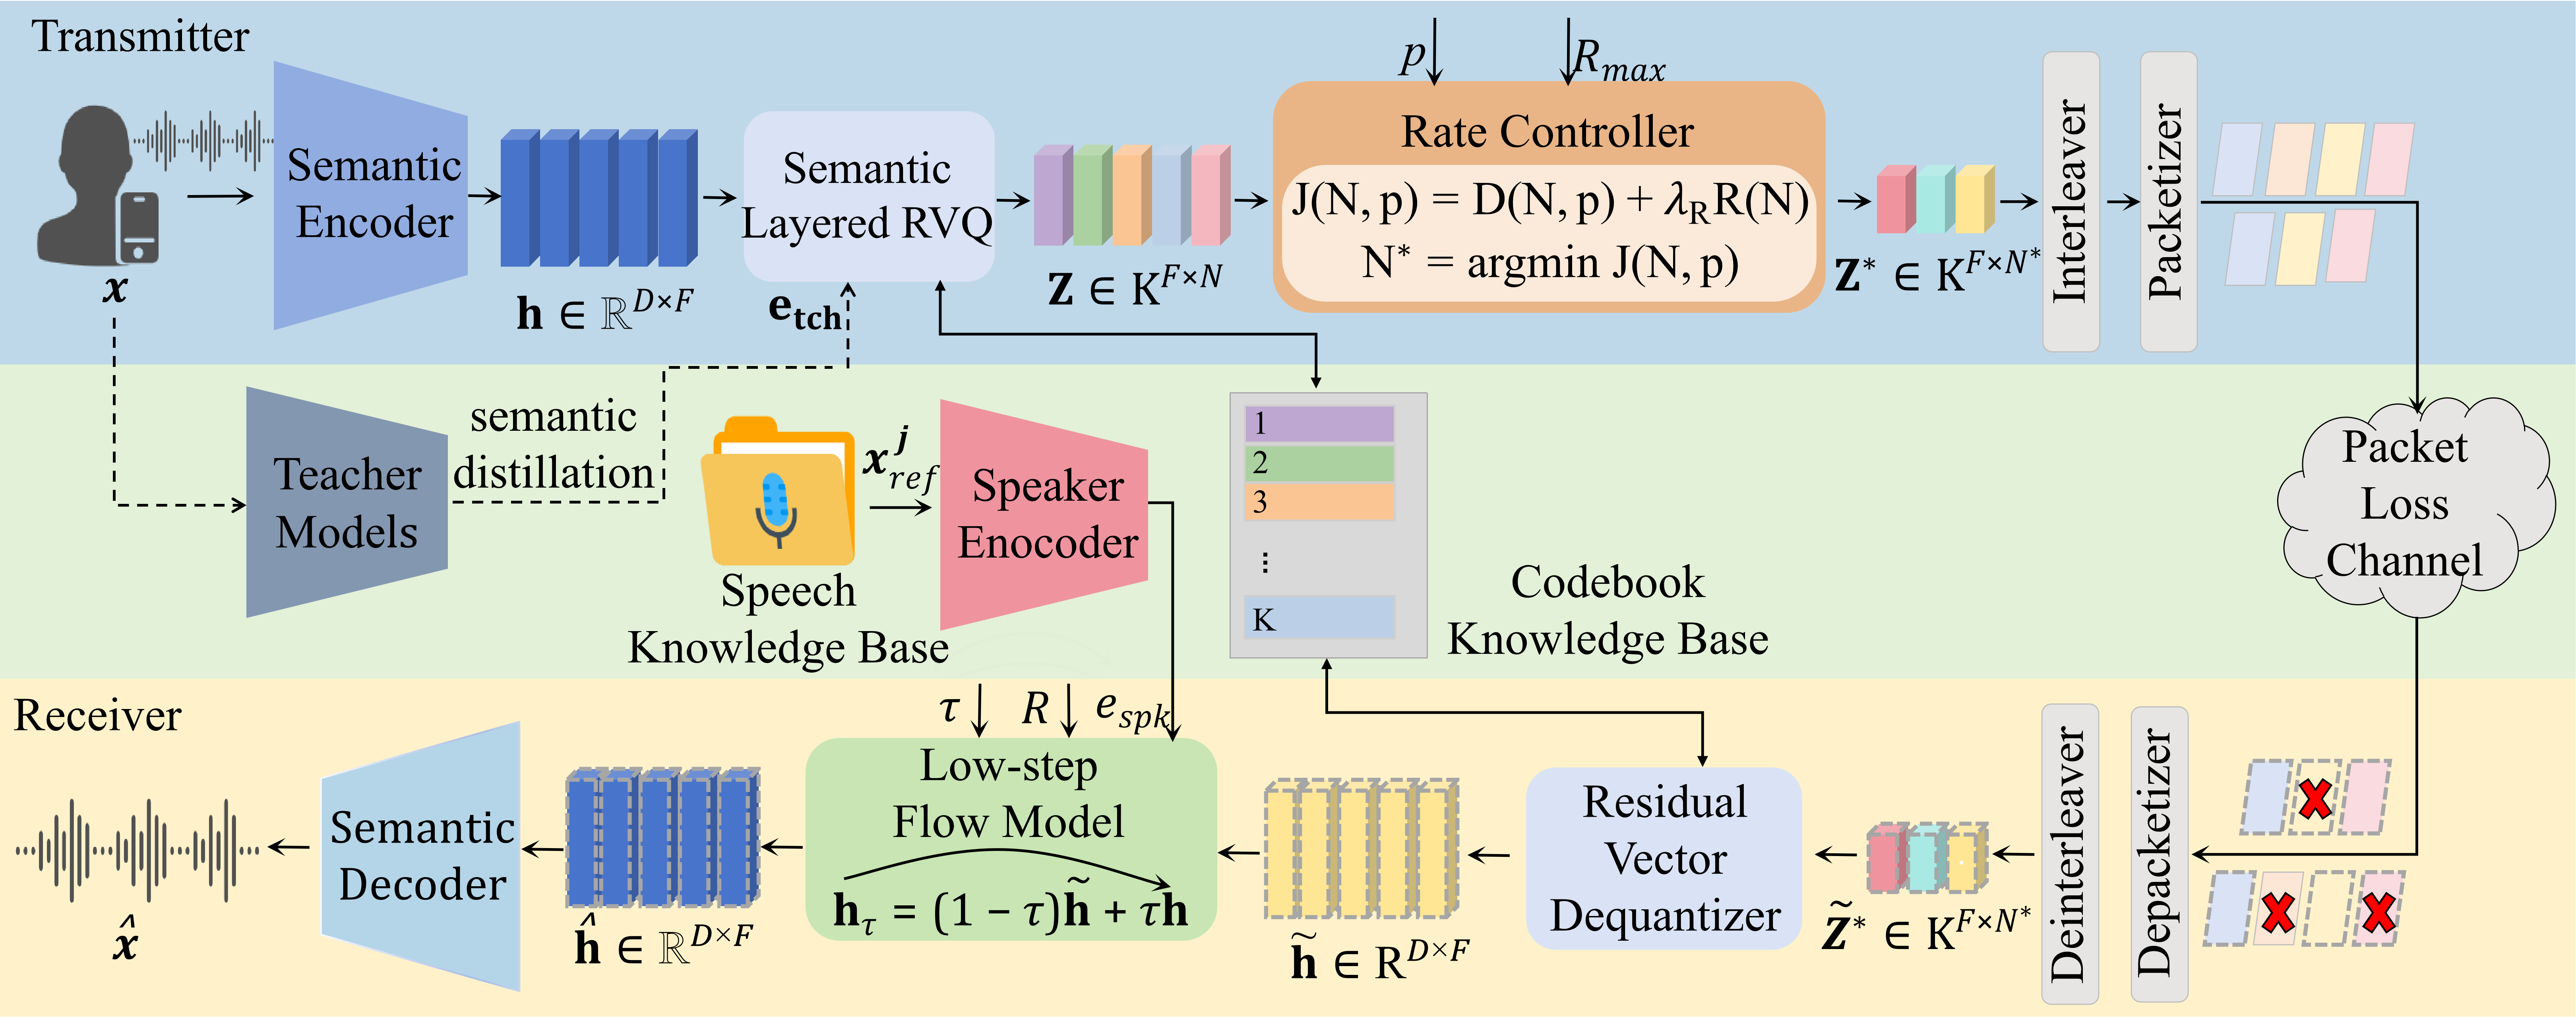
\includegraphics[width=0.92\textwidth]{paper_figs/fig1.png}}
\caption{Overall architecture of the proposed PDSSC system.}
\label{fig:system_model}
\end{figure*}
\section{System Model and Problem Formulation}
This section presents the end-to-end communication model and shows that active bitrate reduction and passive packet erasure lead to the same kind of information loss, so both can be handled by a single receiver-side recovery model.
Fig.~\ref{fig:system_model} illustrates the end-to-end communication setting. We consider a fixed user set $\mathcal{U}=\{1,\ldots,J\}$ of $J$ users communicating over a bandwidth-limited packet-erasure channel. Owing to this stable user population, the receiver maintains a local speech library storing a reference utterance per enrolled user. The transmitter attaches the active user identity, and the receiver retrieves the corresponding same-speaker reference speech $x_{\mathrm{ref}}^{(j)}$ from this library as side information to assist paralinguistic-detail recovery. The overall system therefore consists of (i) a transmitter that generates layered semantic tokens and packetizes them for digital transmission, (ii) a packet-erasure channel, and (iii) a receiver that reconstructs the latent representation and decodes the waveform with side-information-guided recovery. We now describe the transmitter-side layered source representation. Given an input waveform $x$, the transmitter maps it to a latent sequence
\begin{equation}
\mathbf{h}=E_{\phi}(x),\qquad \mathbf{h}\in\mathbb{R}^{D\times F},
\label{eq:enc}
\end{equation}
where $E_{\phi}(\cdot)$ denotes the semantic encoder and the latent spans $D$ feature dimensions over $F$ frames. To obtain a digital source representation compatible with packetized transmission, the continuous latent must be mapped to integer indices, since digital channels transmit discrete symbols rather than floating-point features; quantization into codebook indices further compresses the information to be transmitted. We therefore discretize $\mathbf{h}$ using an 8-layer residual vector quantizer (RVQ) with codebook size $K$, yielding the layered token sequence
\begin{equation}
\mathbf{Z}=\mathcal{Q}(\mathbf{h})=\left[z^{(1)},z^{(2)},\ldots,z^{(N)}\right],
\end{equation}
where $\mathcal{Q}(\cdot)$ denotes RVQ; each $z^{(l)}\in\{0,\ldots,K-1\}^{F}$ selects codewords at layer $l$, and stacking all 8 layers yields the discrete layered index representation $\mathbf{Z}$. The dequantized contributions from all layers are summed to form a complete latent representation, which is then decoded by the shared waveform decoder $D_{\psi}(\cdot)$ to reconstruct the waveform. At the system level, $\mathbf{Z}$ is the digital source description: the first layer carries the transmission-critical semantic content, while the later layers progressively encode speaker-related paralinguistic and residual acoustic detail. The semantic roles of different layers are detailed in Section~III.
\par Thanks to this layered structure, bitrate adaptation is realized by controlling the number of RVQ layers to transmit, denoted $N\in\{1,\ldots,8\}$, with the corresponding transmitted token sequence $\mathbf{Z}^{\star}_{N}=[z^{(1)},\ldots,z^{(N)}]$. The resulting source bitrate is
\begin{equation}
R=N\rho\log_2 K,
\end{equation}
where $R$ denotes the source bitrate, $\rho=f_s/s$ is the latent frame rate, $f_s$ is the sampling rate, and $s$ is the encoder stride. For the configuration used in this work ($f_s=16$~kHz, $s=320$, and $K=1024$), this gives $\rho=50$ frames/s and $R=0.5N$~kbps; thus, $N$ directly determines the operating bitrate. Prior to transmission, the tokens of all layers are interleaved and packetized: a block interleaver of depth $d_{\mathrm{int}}$ spreads the token frames of one block over $d_{\mathrm{int}}$ distinct logical packets. After deinterleaving, the receiver detects which first-layer frames were lost and fills them from their preceding and succeeding neighbors, exploiting the strong temporal correlation of content tokens, while erased supplementary tokens (layers 2--8) are left for the recovery model. The packet-switched channel is modeled as a Gilbert--Elliott two-state Markov channel~\cite{gilbert1960,elliott1963}: the channel state $s_{t}\in\{\mathsf{G},\mathsf{B}\}$ alternates between a good state $\mathsf{G}$, in which packets are delivered, and a bad state $\mathsf{B}$, in which packets are erased; with transition probabilities $\alpha=\Pr(s_{t+1}=\mathsf{B}\mid s_t=\mathsf{G})$ and $\beta=\Pr(s_{t+1}=\mathsf{G}\mid s_t=\mathsf{B})$, the stationary loss probability and the mean burst length are
\begin{equation}
p=\frac{\alpha}{\alpha+\beta},\qquad \bar{T}=\frac{1}{\beta},
\label{eq:ge}
\end{equation}
which follow from the stationary distribution of the two-state chain and from the geometric distribution of the burst length $T$ with mean $\bar{T}=1/\beta$; the channel is therefore fully parameterized by the pair $(p,\bar{T})$.

Without interleaving, the codewords of each token frame are co-located in a single packet, so a burst erases the frame's supplementary detail as a whole and frame-level losses inherit the full burstiness of the channel. Interleaving removes this correlation: the depth-$d_{\mathrm{int}}$ block interleaver spreads the codewords of each token frame over $d_{\mathrm{int}}$ distinct packets, so that a burst erases the frame's supplementary detail if and only if it covers at least one of its codeword positions. As a permutation of packets, it preserves the marginal erasure probability $p$ of every codeword and only reshapes joint erasures. A codeword falls inside a burst with probability $p$, and the burst extends to a codeword $\Delta$ packets away with probability $(1-\beta)^{\Delta}$ by the geometric burst-length distribution, so two codewords are erased by a common burst with probability
\begin{equation}
p(1-\beta)^{\Delta}=p\left(1-\frac{1}{\bar{T}}\right)^{\Delta}\approx p\,e^{-\Delta/\bar{T}},
\label{eq:joint}
\end{equation}

This probability vanishes exponentially as $\Delta$ grows beyond the mean burst length $\bar{T}$: interleaving makes codeword-level erasures approximately independent with common rate $p$, and the frame-level availability masks $\mathbf{M}^{(l)}_{N,p}$ are a sufficient statistic of the channel state at the receiver. After packet loss, depacketization, and deinterleaving, the receiver obtains an incomplete layered token observation $\tilde{\mathbf{Z}}^{\star}_{N,p}$, whose dequantization gives
\begin{equation}
\widetilde{\mathbf{h}}=\mathcal{Q}^{-1}\!\left(\tilde{\mathbf{Z}}^{\star}_{N,p}\right)=\sum_{l=1}^{8}\mathbf{M}^{(l)}_{N,p}\odot \mathbf{h}^{(l)},
\end{equation}
where $\mathcal{Q}^{-1}(\cdot)$ performs RVQ dequantization, $\mathbf{h}^{(l)}$ denotes the dequantized latent contribution of layer $l$, the binary mask $\mathbf{M}^{(l)}_{N,p}$ marks which frames survive layer truncation and packet loss, and $\odot$ denotes element-wise multiplication; $\widetilde{\mathbf{h}}\in\mathbb{R}^{D\times F}$. Therefore, both untransmitted high layers (due to bitrate reduction) and erased packets (due to channel impairment) result in the same mathematical object: an incomplete observation of the complete latent $\mathbf{h}$. This motivates a unified recovery formulation in which the receiver reconstructs a complete latent representation from $\widetilde{\mathbf{h}}$,
\begin{equation}
\widehat{\mathbf{h}}=f_{\theta}(\widetilde{\mathbf{h}},x_{\mathrm{ref}}^{(j)},R),
\end{equation}
where $f_{\theta}(\cdot)$ is the receiver-side latent recovery function. The shared waveform decoder $D_{\psi}(\cdot)$ then maps the completed latent $\widehat{\mathbf{h}}$ back to the reconstructed waveform,
\begin{equation}
\widehat{\mathbf{h}}\in\mathbb{R}^{D\times F},\qquad \hat{x}=D_{\psi}(\widehat{\mathbf{h}}),
\label{eq:dec}
\end{equation}
the decoding counterpart of the encoding map in~\eqref{eq:enc}, which completes the end-to-end transmission chain. With both bitrate reduction and packet erasure cast as incomplete observations of the same latent hierarchy, the central problem becomes to design (i) a digital semantic source representation whose layer ordering aligns with semantic importance, and (ii) a recovery function $f_{\theta}$ that reconstructs the complete latent from such observations, handling both cases within a unified formulation.

\section{Proposed Method}
This section presents the proposed PDSSC framework from both architectural and training perspectives. The method consists of three coupled modules---a semantic-priority layered codec, a receiver-side low-step generative recovery model, and a lightweight channel-adaptive bitrate controller---optimized in three successive stages: Stage I learns the layered codec, Stage II trains the recovery model with the codec frozen, and Stage III fits the controller on RD samples generated by the frozen end-to-end pipeline.

\subsection{Semantic-Priority Layered Codec}
Our codec builds on RVQ~\cite{oord2017vqvae} as its basic quantizer, which decomposes the encoder output into successive residual layers; we use 8 such layers and focus on the 1.0--4.0 kbps operating range. On its own, however, RVQ does not order the layers by semantic importance: content and acoustic characteristics are entangled across layers, so the lowest transmitted layers are not guaranteed to carry the semantic backbone first. Under aggressive bitrate reduction, the retained representation therefore loses information critical to intelligibility.

To impose a semantic ordering on the layer hierarchy, our codec couples the RVQ structure with teacher distillation. As illustrated in Fig.~\ref{fig:codec_arch}, each layer quantizes the residual left by its predecessor, selecting the codeword that minimizes the residual norm,
\begin{equation}
z^{(l)}=\arg\min_{k\in\{0,\ldots,K-1\}}\left\|\mathbf{r}^{(l)}-\mathbf{c}^{(l)}_k\right\|_2^2,
\label{eq:rvq}
\end{equation}
where $\mathbf{r}^{(l)}$ is the residual entering layer $l$, $\{\mathbf{c}^{(l)}_k\}_{k=0}^{K-1}$ is the layer-$l$ codebook, and the selected index $z^{(l)}$ yields the quantized output $\mathbf{h}^{(l)}=\mathbf{c}^{(l)}_{z^{(l)}}$; subtracting it from $\mathbf{r}^{(l)}$ forms the residual $\mathbf{r}^{(l+1)}$ of the next layer. Onto this layered structure, the distillation losses steer the first layer toward the pretrained semantic features and the second toward the pretrained timbre features, so that the lowest two layers capture content and speaker identity as early as possible. The interplay between distillation and residual quantization is twofold: these losses commit the first two layers to the content- and timbre-related parts of the utterance, while the waveform- and spectrogram-level reconstruction losses still require the full stacked representation to recover the original speech. Once the first two layers are committed to matching their teachers, the residual reconstruction error they cannot explain is pushed into the later layers, dominated by prosody, fine spectral detail, and other residual acoustic factors.

The encoder-decoder backbone adopts a SEANet-style architecture~\cite{defossez2023encodec} with a two-layer bidirectional long short-term memory (LSTM) at the encoder output and a two-layer unidirectional LSTM in the decoder, preserving both local acoustic structure and longer-range temporal context; in the notation of Section II, the encoder output has latent dimension $D=1024$. On this backbone, the layer priorities introduced above are realized by two teacher branches. For the first layer, we extract a frame-level semantic teacher $\mathbf{e}_{\mathrm{tch}}$ from a frozen HuBERT model $\mathcal{H}$~\cite{hsu2021hubert}. HuBERT is trained by masked prediction on unlabeled clean speech, so its hidden states emphasize phonetic and linguistic structure while speaker identity, prosody, and other fine acoustic attributes are underrepresented; this content bias makes it a suitable teacher for the lowest transmitted layer, which must carry the semantic backbone. The dequantized feature of the first layer is linearly projected into the teacher's 768-dimensional space, and the semantic distillation loss is imposed between the projected feature $\mathbf{f}^{(1)}\in\mathbb{R}^{768}$ and the teacher representation $\mathbf{e}_{\mathrm{tch}}$, with $\sigma(\cdot)$ denoting the sigmoid function,
\begin{equation}
\mathcal{L}_{\mathrm{dist}}=-\log\sigma\!\left(\cos(\mathbf{f}^{(1)},\mathbf{e}_{\mathrm{tch}})\right),
\end{equation}

For the second layer, we adopt a frozen ECAPA-TDNN model $\mathcal{E}$~\cite{desplanques2020ecapa} as the timbre teacher, separating speaker identity from the semantic backbone captured by the first layer. ECAPA-TDNN is a speaker-verification architecture trained purely for speaker discrimination, so it learns to discard content, prosody, and other factors that do not help distinguish speakers, and its embedding concentrates on speaker identity alone---exactly the factor we want the second layer to encode. The dequantized feature of the second layer is linearly projected to the ECAPA-TDNN embedding dimension and temporally pooled into a single utterance-level vector, matching the teacher's granularity; the timbre distillation loss is then imposed as
\begin{equation}
\mathcal{L}_{\mathrm{tim}}=-\log\sigma\!\left(\cos(\mathbf{f}^{(2)},\mathbf{e}_{\mathrm{tim}})\right),
\end{equation}
where $\mathbf{f}^{(2)}$ is the projected second-layer feature and $\mathbf{e}_{\mathrm{tim}}$ is the teacher timbre embedding. The two distillation terms are combined into a single objective with deliberately asymmetric weights,
\begin{equation}
\mathcal{L}_{\mathrm{distill}}=\lambda_{\mathrm{dist}}\mathcal{L}_{\mathrm{dist}}+\lambda_{\mathrm{tim}}\mathcal{L}_{\mathrm{tim}},
\label{eq:distill}
\end{equation}
The weights $\lambda_{\mathrm{dist}}$ and $\lambda_{\mathrm{tim}}$ are set with $\lambda_{\mathrm{dist}}>\lambda_{\mathrm{tim}}$: intelligibility-critical content must be guaranteed in the lowest transmitted layer even under the most aggressive bitrate reduction, while the second-layer speaker identity is refined on top of an already meaningful semantic backbone, so the overall distillation budget is tilted toward the first-layer semantic term rather than split equally.
Beyond the two distillation terms, the codec keeps the standard reconstruction and regularization objectives: $\mathcal{L}_{\mathrm{rec}}=\|x-\hat{x}\|_1$ is the waveform reconstruction loss, $\mathcal{L}_{\mathrm{mel}}$ is the multi-scale mel-spectrogram loss, $\mathcal{L}_{\mathrm{commit}}$ is the RVQ commitment loss, and $\mathcal{L}_{\mathrm{adv}}$ and $\mathcal{L}_{\mathrm{fm}}$ are the adversarial and discriminator feature-matching losses. Stage I jointly trains the encoder, RVQ, and decoder end to end by minimizing
\begin{align}
\mathcal{L}_{\mathrm{codec}}&=\lambda_{\mathrm{adv}}\mathcal{L}_{\mathrm{adv}}+\lambda_{\mathrm{fm}}\mathcal{L}_{\mathrm{fm}}+
\lambda_{\mathrm{mel}}\mathcal{L}_{\mathrm{mel}}+\lambda_{\mathrm{rec}}\mathcal{L}_{\mathrm{rec}}\notag\\
&\quad+\lambda_{\mathrm{q}}\mathcal{L}_{\mathrm{commit}}+\mathcal{L}_{\mathrm{distill}},
\label{eq:codec_loss}
\end{align}
where the scalar weights $\lambda_{\mathrm{adv}},\lambda_{\mathrm{fm}},\lambda_{\mathrm{mel}},\lambda_{\mathrm{rec}},\lambda_{\mathrm{q}}$ balance the adversarial, spectral, reconstruction, and commitment objectives, and $\mathcal{L}_{\mathrm{distill}}$ is the joint distillation objective in~\eqref{eq:distill}. Algorithm~\ref{alg:distill} outlines the corresponding forward training step, in which each mini-batch is encoded, quantized layer by layer, and scored by the two teacher projections before the parameter update.
After Stage I, the trained encoder-decoder is frozen as the shared front end for both transmission and receiver-side recovery.

\begin{algorithm}[tb]\small
\setlength{\baselineskip}{12.0pt}
\caption{Forward Training Step of the Layered Codec}
\label{alg:distill}
\begin{algorithmic}[1]
\STATE \textbf{Input:} mini-batch utterances $\{x_i\}$; frozen semantic teacher $\mathcal{H}$ and timbre teacher $\mathcal{E}$; codec parameters $(\phi,\{\mathcal{C}^{(l)}\},\psi)$
\STATE \textbf{Output:} updated codec parameters and the joint distillation loss $\mathcal{L}_{\mathrm{distill}}$
\STATE $\{\mathbf{h}_i\}\leftarrow E_{\phi}(\{x_i\})$ \COMMENT{semantic encoding}
\STATE $\{\mathbf{r}^{(1)}_i\}\leftarrow\{\mathbf{h}_i\}$ \COMMENT{the first stage quantizes the encoder output}
\FOR{$l=1$ \TO $8$}
\STATE $\{z^{(l)}_i\}\leftarrow\arg\min_{z}\left\|\mathbf{r}^{(l)}_i-\mathbf{c}^{(l)}_{z}\right\|$ \COMMENT{RVQ step in~\eqref{eq:rvq}}
\STATE $\{\mathbf{h}^{(l)}_i\}\leftarrow\left\{\mathbf{c}^{(l)}_{z^{(l)}_i}\right\}$ \COMMENT{quantized output of layer $l$}
\STATE $\{\mathbf{r}^{(l+1)}_i\}\leftarrow\{\mathbf{r}^{(l)}_i\}-\left\{\mathbf{c}^{(l)}_{z^{(l)}_i}\right\}$
\ENDFOR
\STATE $\{\mathbf{e}_{\mathrm{tch},i}\}\leftarrow\mathcal{H}(\{x_i\})$ \COMMENT{frozen teacher features}
\STATE $\{\mathbf{e}_{\mathrm{tim},i}\}\leftarrow\mathcal{E}(\{x_i\})$
\STATE $\{\mathbf{f}^{(1)}_i\}\leftarrow\mathrm{Proj}_1\!\left(\{\mathbf{h}^{(1)}_i\}\right)$ \COMMENT{projection to the semantic space}
\STATE $\{\mathbf{f}^{(2)}_i\}\leftarrow\mathrm{Pool}\!\left(\mathrm{Proj}_2\!\left(\{\mathbf{h}^{(2)}_i\}\right)\right)$ \COMMENT{pooling to the timbre space}
\STATE $\mathcal{L}_{\mathrm{dist}}\leftarrow-\log\sigma\!\left(\cos(\mathbf{f}^{(1)},\mathbf{e}_{\mathrm{tch}})\right)$ \COMMENT{semantic alignment}
\STATE $\mathcal{L}_{\mathrm{tim}}\leftarrow-\log\sigma\!\left(\cos(\mathbf{f}^{(2)},\mathbf{e}_{\mathrm{tim}})\right)$ \COMMENT{timbre alignment}
\STATE $\mathcal{L}_{\mathrm{distill}}\leftarrow\lambda_{\mathrm{dist}}\mathcal{L}_{\mathrm{dist}}+\lambda_{\mathrm{tim}}\mathcal{L}_{\mathrm{tim}}$ \COMMENT{$\lambda_{\mathrm{dist}}>\lambda_{\mathrm{tim}}$}
\STATE $\mathcal{L}_{\mathrm{codec}}\leftarrow\lambda_{\mathrm{adv}}\mathcal{L}_{\mathrm{adv}}+\lambda_{\mathrm{fm}}\mathcal{L}_{\mathrm{fm}}+\lambda_{\mathrm{mel}}\mathcal{L}_{\mathrm{mel}}+\lambda_{\mathrm{rec}}\mathcal{L}_{\mathrm{rec}}+\lambda_{\mathrm{q}}\mathcal{L}_{\mathrm{commit}}+\mathcal{L}_{\mathrm{distill}}$
\STATE Update $(\phi,\{\mathcal{C}^{(l)}\},\psi)$ by gradient descent on $\mathcal{L}_{\mathrm{codec}}$
\STATE \textbf{return} updated codec parameters
\end{algorithmic}
\end{algorithm}

\begin{figure*}[tb]
\centering
\makebox[\textwidth][c]{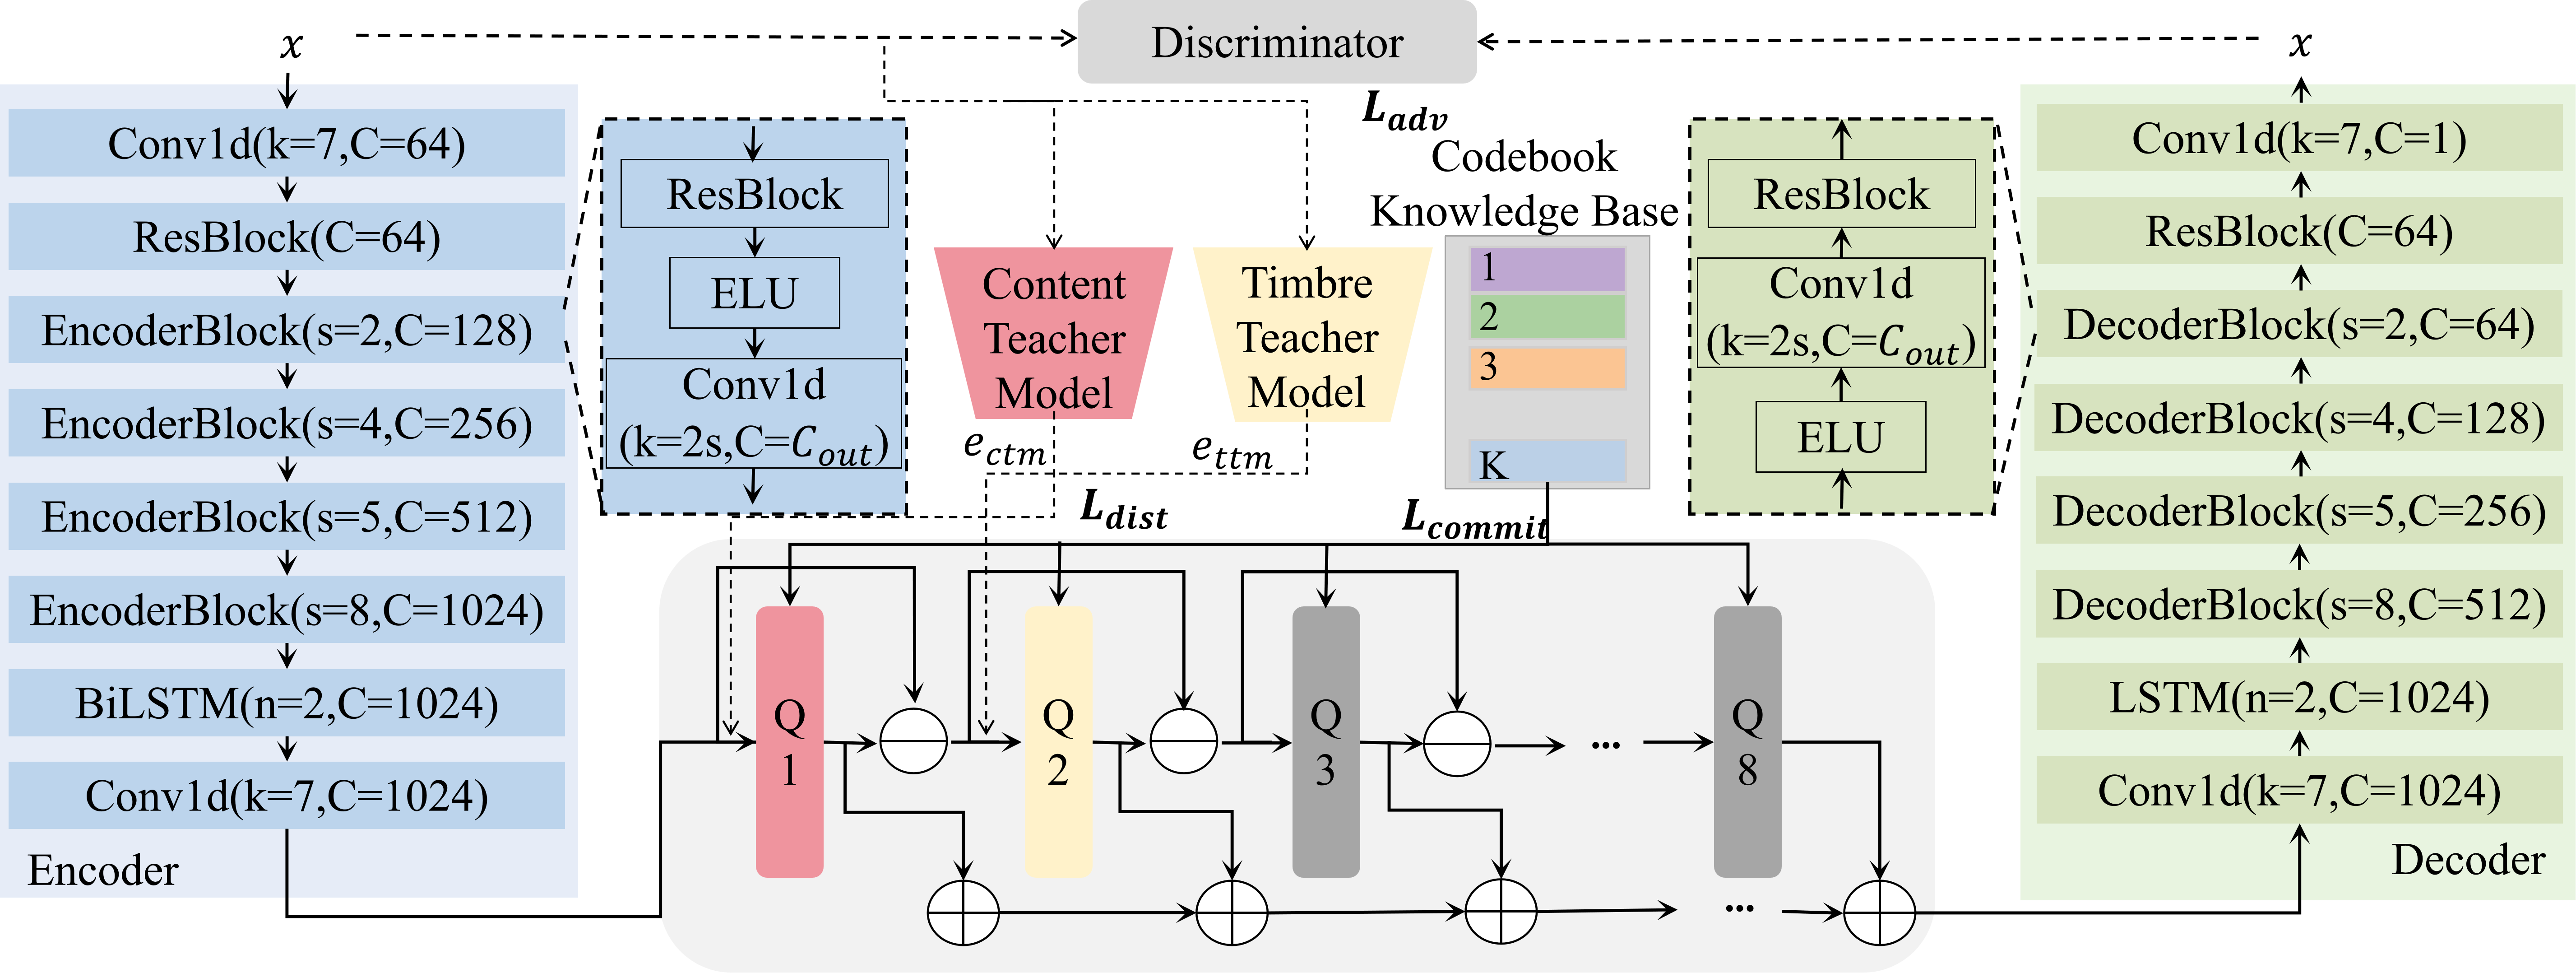
\includegraphics[width=0.96\textwidth]{paper_figs/fig2.png}}
\caption{Architecture of the semantic-priority layered codec.}
\label{fig:codec_arch}
\end{figure*}

\subsection{Low-Step Generative Recovery Model}
When higher layers are untransmitted or erased, direct decoding of the received partial description cannot recover complete speech: the missing high-layer detail must be regenerated from the surviving representation. High-fidelity generative models, however, are typically expensive: large language model (LLM)-based speech generation demands very large models, and diffusion-style generation requires many sampling steps, so the resulting memory footprint and inference latency conflict with the strict real-time budget of interactive speech communication. To avoid this cost, as illustrated in Fig.~\ref{fig:timbreflow_arch}, we implement the recovery as a low-step generative model in flow-matching form~\cite{lipman2023flow}. Conditioned on the side information already available at the receiver---the preserved semantic backbone and the speaker reference embedding---the model restores the missing detail with only a few integration steps, keeping inference fast enough for real-time operation while retaining high fidelity.

At the receiver, lost frames of the first-layer semantic backbone are filled from their neighbors, while the missing higher layers---prosody, timbre, and residual spectral detail---are regenerated by the generative model. For this recovery we adopt flow matching, which---unlike diffusion models that learn a stepwise denoising process---learns the velocity direction of the trajectory, i.e., the vector field pointing from the incomplete latent toward the complete one. This velocity field is conditioned on the side information already available at the receiver: the preserved semantic backbone anchors the direction of recovery, and since prosody and timbre are largely consistent across a speaker's utterances, a reference utterance from the same speaker supplies precisely the missing speaker-related factors, steering the regenerated detail toward the target speaker's acoustic characteristics. Conditioning on these factors improves the fidelity of the regenerated detail and keeps it accurate even when only a few integration steps are taken, so that inference is accelerated accordingly.

Specifically, for the active speaker $j$, the receiver retrieves the pre-stored reference utterance $x_{\mathrm{ref}}^{(j)}$ from the local speech library and encodes it with a pretrained reference encoder to obtain the speaker embedding $\mathbf{e}_{\mathrm{spk}}$. Since the embedding is derived locally from stored speech, it costs no transmission bandwidth and is unaffected by channel distortion. Unlike the second-layer timbre teacher, whose representation concentrates on speaker identity alone, the recovery conditioning must guide reconstruction of the full missing residual---not only timbre but also prosody, spectral fine structure, and other acoustic detail spread across layers 2--8. We therefore adopt a frozen WavLM model~\cite{chen2022wavlm} as the reference encoder. WavLM extends HuBERT with a denoising-based masked prediction objective in which noise and overlapping speech are deliberately added before masking, so its contextualized hidden states jointly encode speaker, prosody, and fine acoustic characteristics rather than a single factor. Although its representation also carries content information, this redundancy is harmless: the semantic backbone is already preserved in the received first-layer latent, so the trainable projection can focus on recovery-relevant non-content factors. On top of the frozen WavLM backbone, a trainable projection and pooling layer maps the hidden states to a compact embedding, which is combined with a 128-dimensional sinusoidal time embedding and the bitrate condition $R$ into a unified conditioning signal that modulates the residual blocks of the flow network.

In Stage II, the codec is frozen and the channel simulator is enabled, so each training sample is generated on the fly: the codec produces the complete latent $\mathbf{h}$, and jointly sampled bitrate and packet-loss conditions yield the incomplete counterpart $\widetilde{\mathbf{h}}$. A continuous time variable $\tau\sim\mathcal{U}(0,1)$ is then drawn, and a straight-line interpolation defines the intermediate state along the recovery trajectory,
\begin{equation}
\mathbf{h}_{\tau}=(1-\tau)\widetilde{\mathbf{h}}+\tau\mathbf{h},
\qquad
\mathbf{v}^{\star}=\mathbf{h}-\widetilde{\mathbf{h}},
\end{equation}
whose time derivative is the target velocity; sampling $\tau$ over $[0,1]$ lets the network learn the full time-conditioned velocity field. Using the frame-wise availability masks $\mathbf{M}^{(l)}_{N,p}$ introduced in Section~II, the same velocity can be rewritten over the frame-level layer outputs $\mathbf{h}^{(l)}$ to expose its layered structure,
\begin{equation}
\mathbf{v}^{\star}=
\sum_{l=1}^{8}\left(1-\mathbf{M}^{(l)}_{N,p}\right)\odot \mathbf{h}^{(l)},
\end{equation}
This decomposition shows the velocity points exactly toward the missing residual components, so the model restores layered detail on top of the preserved semantic backbone rather than regenerating the representation from scratch. The network $F_{\theta}$, a 1-D U-Net assembled from the shared residual blocks, with downsampling, middle attention, and upsampling stages connected by skip connections, takes the interpolated latent $\mathbf{h}_{\tau}$ as input; conditioned on the continuous time $\tau$, the speaker embedding $\mathbf{e}_{\mathrm{spk}}$, and the bitrate $R$, it predicts the conditional vector field
\begin{equation}
\mathbf{v}_{\theta}=F_{\theta}(\mathbf{h}_{\tau},\tau,\mathbf{e}_{\mathrm{spk}},R),
\end{equation}
which is supervised by the flow-matching objective
\begin{equation}
\mathcal{L}_{\mathrm{flow\text{-}comp}}=\mathbb{E}\!\left[w(R)\left\|\mathbf{v}_{\theta}-\mathbf{v}^{\star}\right\|_2^2\right]+\lambda_{\mathrm{stft}}\mathcal{L}_{\mathrm{mrstft}},
\end{equation}
The spectral term $\lambda_{\mathrm{stft}}\mathcal{L}_{\mathrm{mrstft}}$, a multi-resolution STFT reconstruction loss between the waveform decoded from the recovered latent and the target waveform, constrains local spectral continuity and fine acoustic detail. To emphasize harder low-rate cases, the rate-dependent weight is set as $w(R)=\max\!\left(1,\,(5-R)/2\right)$, i.e., 2.0 at 1.0 kbps decreasing to 1.0 at 3.0 kbps and above. During Stage II, $R$ is sampled from 1.0 to 4.0 kbps with explicit bias toward the lowest-rate regime and the packet loss probability from 0 to 30\%, with erasure injected only into the supplementary residual information. Training a single model jointly over all rate points with $R$ as a conditioning input realizes rate adaptation with one model instance, so that no rate-specific models need to be trained or switched between, simplifying deployment.

At inference time, a low-step Euler solver recovers the latent representation:
\begin{equation}
\widehat{\mathbf{h}}^{(k+1)}=\widehat{\mathbf{h}}^{(k)}+\Delta \tau\,F_{\theta}(\widehat{\mathbf{h}}^{(k)},\tau_k,\mathbf{e}_{\mathrm{spk}},R),
\end{equation}
with step size $\Delta\tau$ over $S$ steps indexed by $k=0,\ldots,S-1$, initialized from the received incomplete latent $\widehat{\mathbf{h}}^{(0)}=\widetilde{\mathbf{h}}$. Algorithm~\ref{alg:recovery} outlines the receiver-side recovery procedure, in which the surviving codewords are dequantized and reassembled into the incomplete latent $\widetilde{\mathbf{h}}$ (with first-layer gaps filled from neighboring frames), the speaker embedding $\mathbf{e}_{\mathrm{spk}}$ is extracted from the reference utterance, and the low-step Euler solver, conditioned on the step time, the speaker embedding, and the bitrate $R^{\star}$, iterates the learned velocity field from $\widehat{\mathbf{h}}^{(0)}=\widetilde{\mathbf{h}}$ to complete the missing layers before waveform decoding.

\begin{algorithm}[tb]\small
\setlength{\baselineskip}{12.0pt}
\caption{Receiver-Side Recovery of PDSSC}
\label{alg:recovery}
\begin{algorithmic}[1]
\STATE \textbf{Input:} surviving codewords of the received description (bitrate $R^{\star}$); same-speaker reference utterance $x_{\mathrm{ref}}^{(j)}$; step count $S$ with step size $\Delta\tau$
\STATE \textbf{Output:} recovered waveform $\hat{x}$
\STATE Dequantize the surviving codewords and reassemble the incomplete latent $\widetilde{\mathbf{h}}$ under the masks $\mathbf{M}^{(l)}_{N,p}$ \COMMENT{first-layer gaps filled from neighbors}
\STATE $\mathbf{e}_{\mathrm{spk}}\leftarrow\mathrm{WavLM}_{\mathrm{proj}}(x_{\mathrm{ref}}^{(j)})$ \COMMENT{speaker reference embedding}
\STATE $\widehat{\mathbf{h}}^{(0)}\leftarrow\widetilde{\mathbf{h}}$
\FOR{$k=0$ \TO $S-1$}
\STATE $\tau_k\leftarrow k\,\Delta\tau$ \COMMENT{time condition of step $k$}
\STATE $\widehat{\mathbf{h}}^{(k+1)}\leftarrow\widehat{\mathbf{h}}^{(k)}+\Delta\tau\,F_{\theta}(\widehat{\mathbf{h}}^{(k)},\tau_{k},\mathbf{e}_{\mathrm{spk}},R^{\star})$ \COMMENT{low-step Euler update}
\ENDFOR
\STATE $\hat{x}\leftarrow D_{\psi}(\widehat{\mathbf{h}}^{(S)})$ \COMMENT{decode from the recovered latent}
\STATE \textbf{return} $\hat{x}$
\end{algorithmic}
\end{algorithm}

\begin{figure}[tb]
\centering
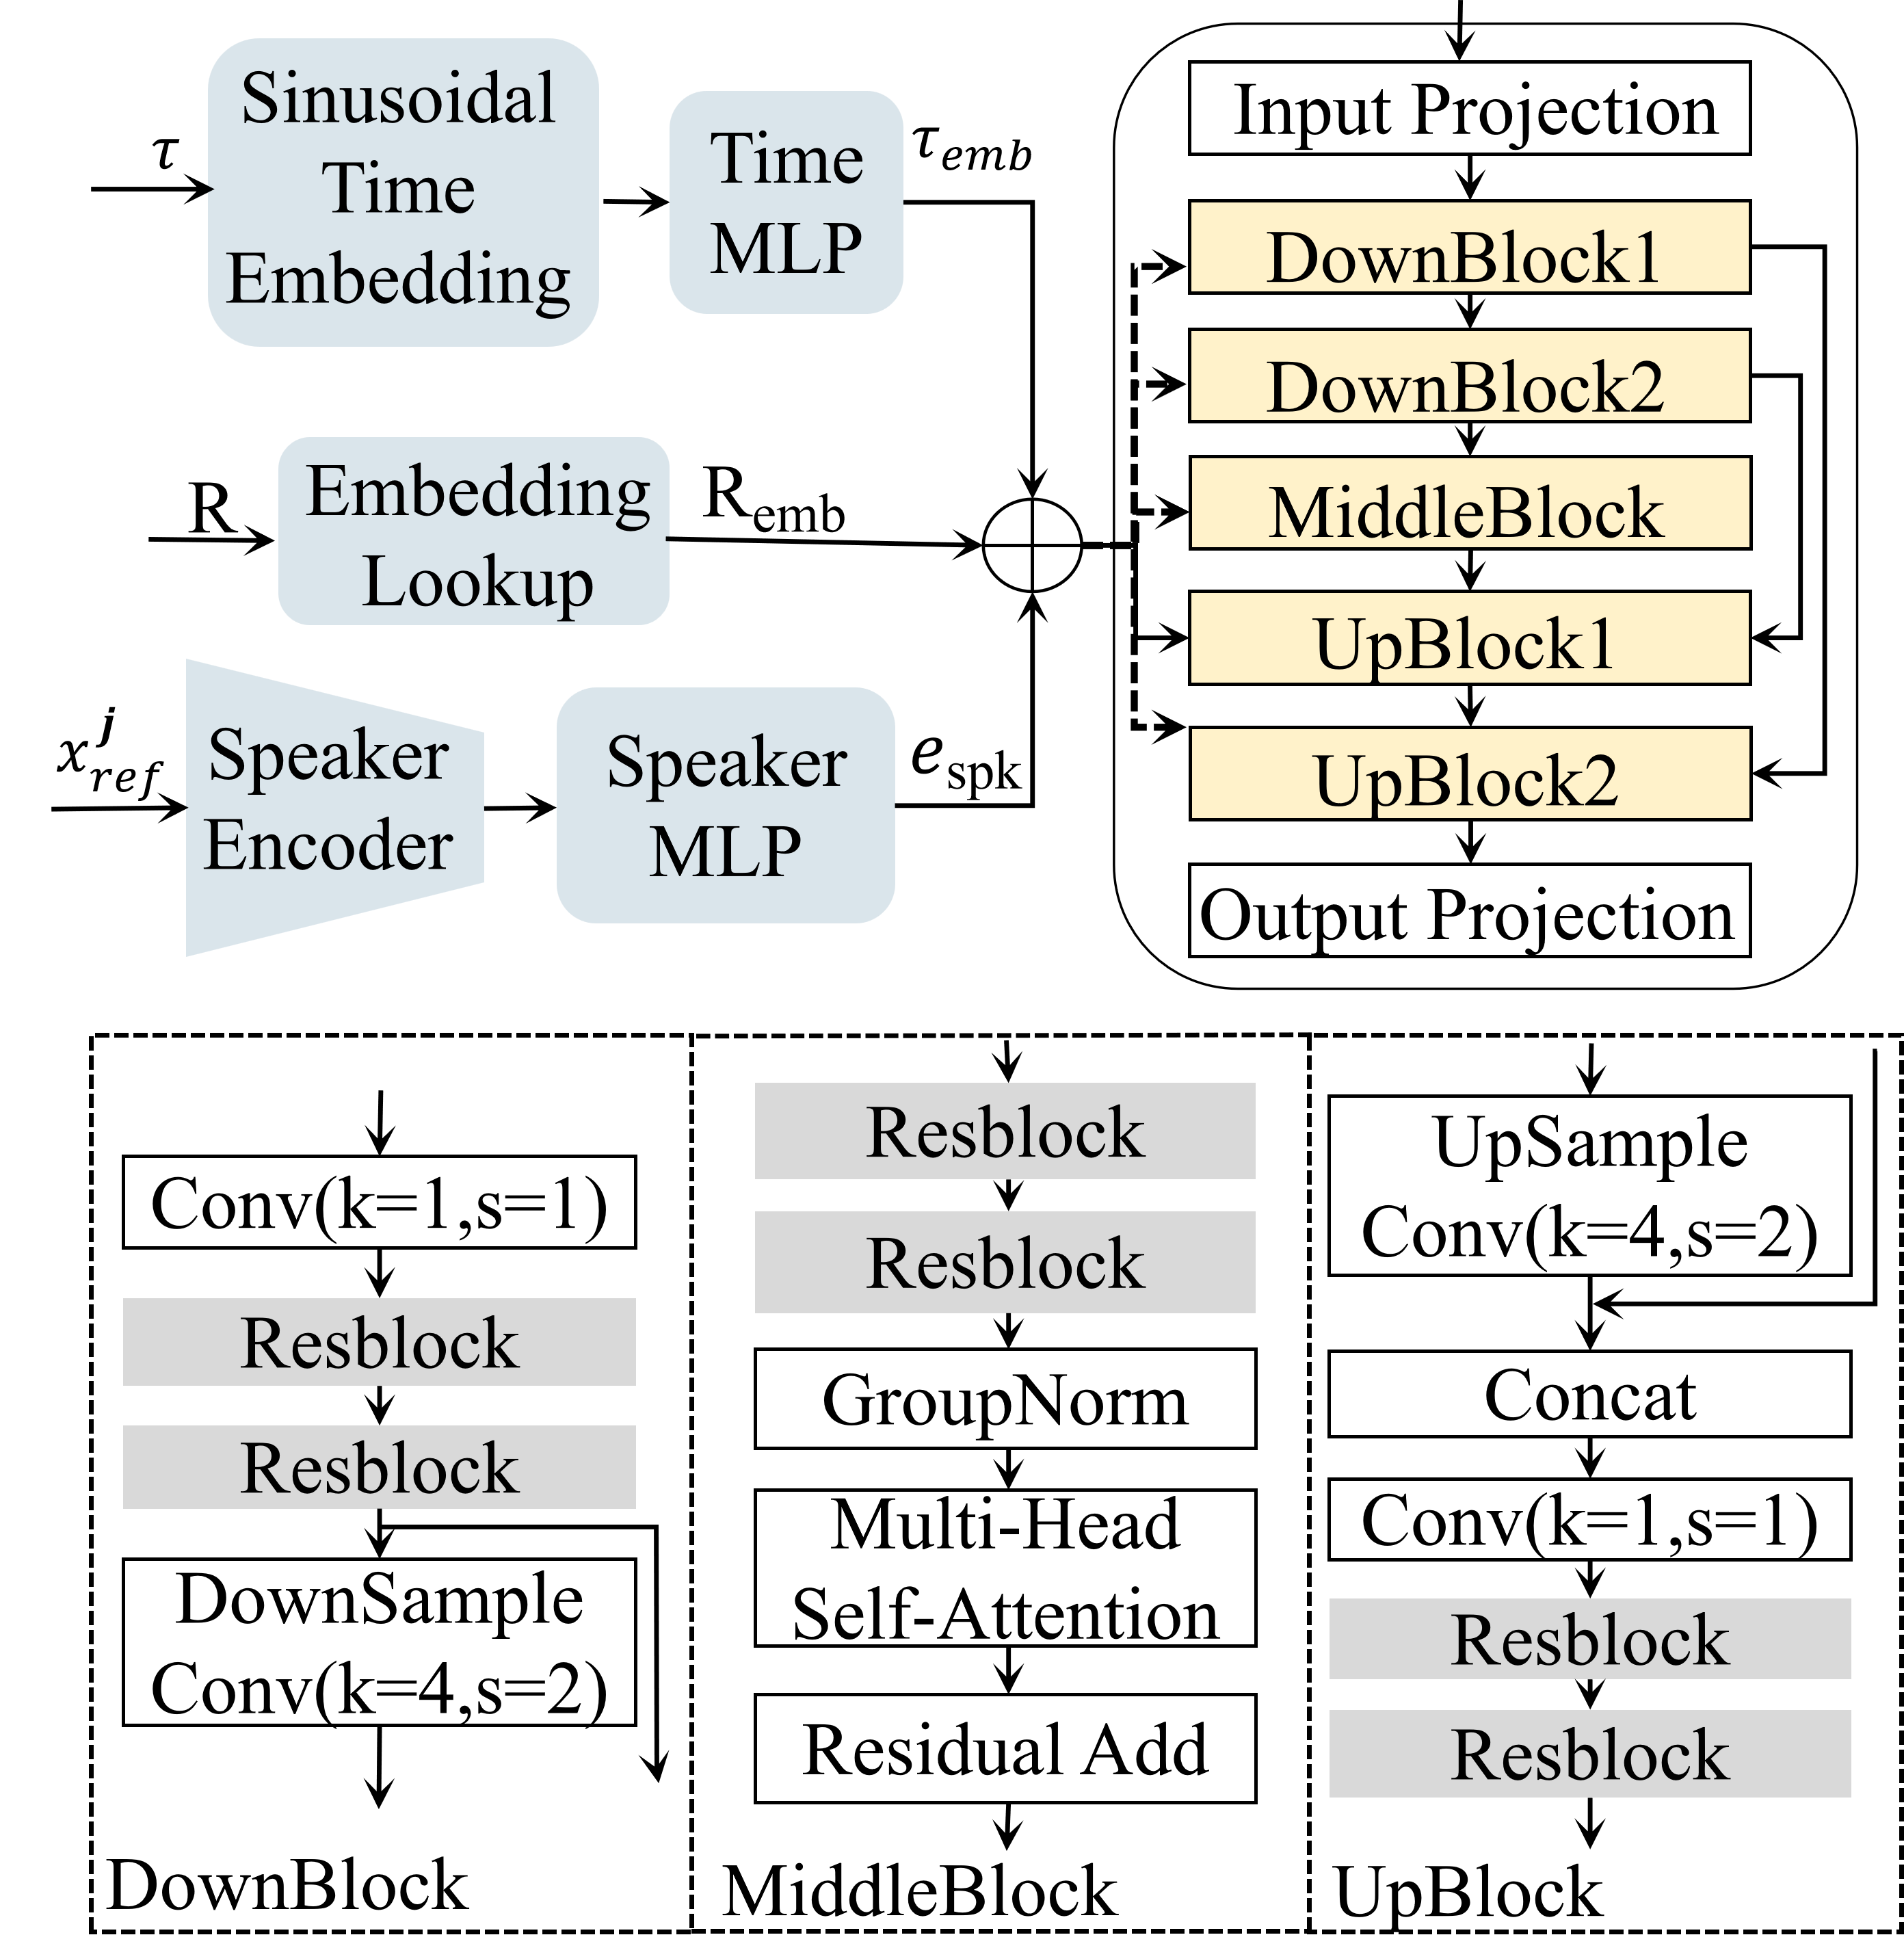
\includegraphics[width=0.93\linewidth]{paper_figs/fig3.png}
\caption{Architecture of the low-step generative recovery module.}
\label{fig:timbreflow_arch}
\end{figure}

Both stages of PDSSC are assembled from a common residual block, whose internal structure is shown in Fig.~\ref{fig:resblock}: a residual branch of two stacked 1-D convolutions learns the update to the input, which is preserved by an identity skip connection and added back to form the output. In Stage~I, this unit forms the SEANet-style backbone of the layered codec; in Stage~II, it becomes the building block of the recovery network's 1-D U-Net, extended with a feature-wise linear modulation (FiLM) layer for conditional generation. Reusing one residual design across both stages keeps the parameterization compact.

\begin{figure}[tb]
\centering
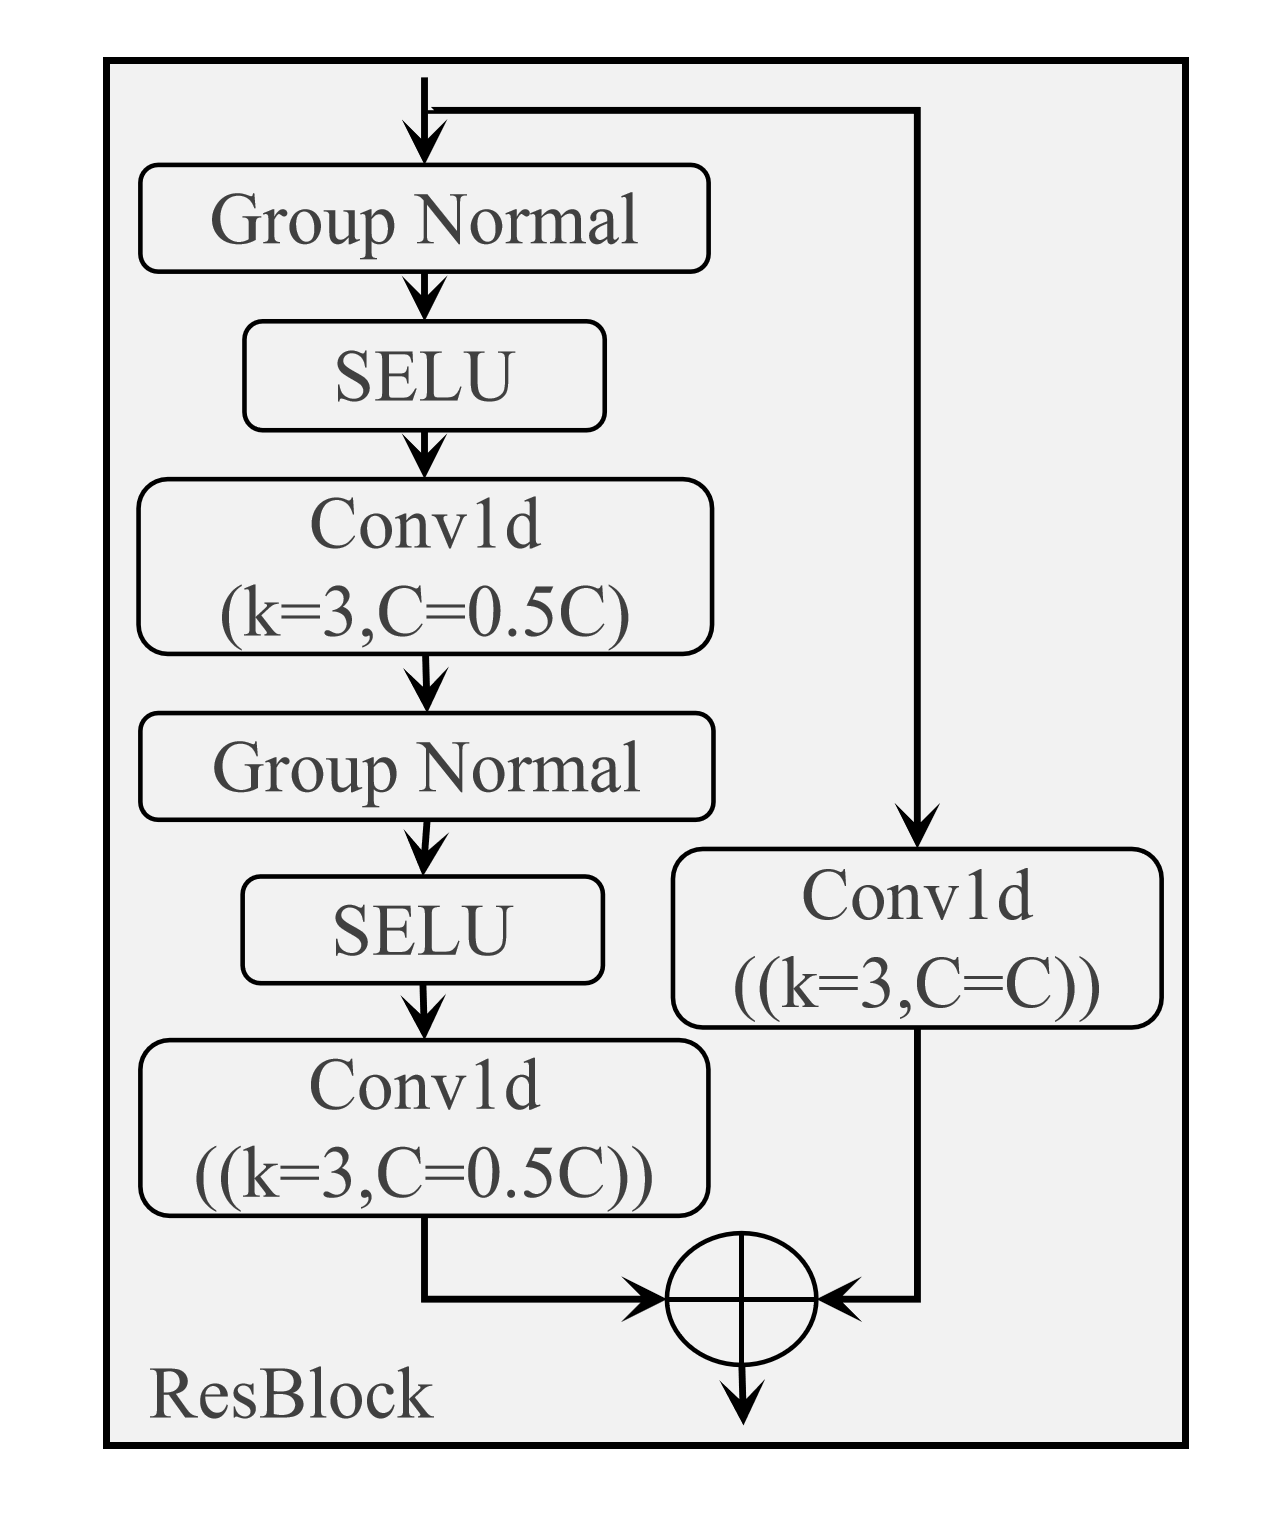
\includegraphics[width=0.63\linewidth]{paper_figs/fig9.png}
\caption{Internal structure of the shared residual block.}
\label{fig:resblock}
\end{figure}
\subsection{Channel-Adaptive Bitrate Control}
Thanks to the layered representation and the receiver-side recovery model, PDSSC operates over a range of rates from 1.0 to 4.0 kbps, where each rate corresponds to transmitting a different number of leading RVQ layers. The choice of operating rate, however, must follow the time-varying channel state: fixing one rate wastes bandwidth when the channel is good and sacrifices quality when it deteriorates, while manual switching cannot track such variation reliably. We therefore design a lightweight channel-adaptive bitrate controller that makes this decision automatically. With the codec and recovery model frozen after Stage~II, the end-to-end rate-distortion (RD) tradeoff is determined by the channel state and the rate budget, so channel adaptation calls for a decision rule over this surface rather than any system retraining. We train a small policy network to learn this rule from RD samples collected on the frozen pipeline, so that the learned rule generalizes across the full loss-rate and rate-budget space at negligible inference cost.

Given the packet loss rate $p$ and the available source-rate budget $R_{\max}$, the controller minimizes the RD cost. To quantify this cost, let $\widetilde{x}_{x,N,p}$ denote the reconstructed waveform for utterance $x$ transmitted with $N$ layers over a channel with loss rate $p$, after channel degradation and receiver-side recovery; the recovered quality is $\widetilde{D}(x,N,p)=d\!\left(\widetilde{x}_{x,N,p},x\right)$, where $d(\cdot,\cdot)$ denotes the distortion metric used to score reconstruction quality. The RD cost of transmitting $N$ layers is then
\begin{equation}
\mathcal{J}(x,N,p)=\widetilde{D}(x,N,p)+\lambda_R R(N),
\label{eq:jcost}
\end{equation}
where $N\in\{2,3,\ldots,8\}$ denotes a candidate number of transmitted layers, corresponding to 1.0--4.0 kbps in steps of 0.5 kbps, $R(N)$ is the bitrate of transmitting $N$ leading layers (i.e., $0.5N$ kbps in our configuration), and $\lambda_R$ balances the bitrate cost against the distortion. At deployment, however, the distortion value $\widetilde{D}(x,N,p)$ cannot be obtained, since computing it requires the original waveform $x$, which is unavailable at the receiver; we therefore train a predictor $D_\omega(N,p)$ to estimate the recovered quality from the layer count and loss rate.

To train the controller, we sample utterances and packet loss rates and run the frozen end-to-end pipeline over all candidate layer counts, recording the recovered quality $\widetilde{D}(x,N,p)$ defined above for each $(x,p)$; the sampled loss rate serves as the channel estimate at deployment. The controller is parameterized by a small policy network $\pi_{\omega}$ with parameters $\omega$, which takes $p$ together with $R_{\max}$ as input and outputs a score over candidate layer counts. During training, the score vector is converted to a soft decision distribution
\begin{equation}
\pi_{\omega}(N|p,R_{\max})=\frac{\exp(-D_\omega(N,p)/T_c)}{\sum_{n=2}^{8}\exp(-D_\omega(n,p)/T_c)},
\end{equation}
where $T_c$ is a temperature parameter and $D_\omega(N,p)$ is the distortion predicted by the policy network; using the predicted distortion rather than the recovered quality $\widetilde{D}$ keeps the training signal differentiable for end-to-end policy learning. We then optimize the expected RD objective
\begin{equation}
\mathcal{L}_{\mathrm{ctrl}}=\mathbb{E}_{x,p}\!\Big[\sum_{N=2}^{8}\pi_{\omega}(N|p,R_{\max})\,\mathcal{J}(x,N,p)\Big].
\label{eq:ctrl_loss}
\end{equation}
Each evaluation yields an RD sample $(x,N,p,\widetilde{D}(x,N,p))$; in Stage III, the policy network and the distortion predictor are trained jointly over RD samples generated by the frozen end-to-end system---the policy by minimizing the expected RD cost in~\eqref{eq:ctrl_loss}, and the predictor $D_\omega$ by regression onto the recovered quality $\widetilde{D}$. At deployment, the trained policy $\pi_\omega$ selects the layer count $N^{\star}$ directly from the current loss rate and rate budget, yielding the operating bitrate $R^{\star}=0.5N^{\star}$~kbps, with the predictor $D_\omega$ supplying the quality estimate---adding negligible inference overhead while keeping the system responsive to time-varying channel conditions.

\section{Experimental Results and Analysis}
We evaluate PDSSC from four complementary perspectives: quality-bitrate tradeoff, packet-loss robustness, component ablation, and qualitative reconstruction and deployment efficiency. All experiments are conducted on LibriSpeech~\cite{panayotov2015librispeech}, with the codec and recovery model trained on \texttt{train-clean-100} and the main results reported on \texttt{test-clean}. Training uses four NVIDIA A40 GPUs in about 50 hours, while evaluation and latency measurement are performed on a single NVIDIA RTX 3090 workstation. We compare against the conventional codecs AAC and Opus, the neural codec EnCodec, and the recent low-bitrate semantic baseline ESC~\cite{gu2024esc}; to ensure a fair comparison under packet-loss channels, all baselines are equipped with their respective packet-loss-resilience tools, i.e., low-bitrate redundancy (LBRR) for Opus and low-frame-rate packet loss concealment (LFR-PLC) for AAC, EnCodec, and ESC.

\subsection{Quality-Bitrate Tradeoff}

We first analyze the quality-bitrate tradeoff, as shown in Fig.~\ref{fig:rate}. PDSSC is evaluated from 1.0 to 4.0 kbps at 0.5 kbps intervals, with ViSQOL~\cite{chinen2020visqolv3} measuring objective speech quality and UTMOS~\cite{saeki2022utmos} perceptual naturalness. On both metrics PDSSC rises steeply from the lowest bitrate and reaches its plateau the fastest. Compared with the conventional codecs AAC and Opus, which remain nearly flat across the tested range, PDSSC delivers higher quality at a much lower bitrate, reaching the level they approach only at several times the rate: its ViSQOL of 4.14 at 2.0 kbps already exceeds Opus at 8.0 kbps (3.63), and its UTMOS of 3.60 at 2.0 kbps surpasses the best values of Opus (2.64) and AAC (2.90). The advantage is most pronounced below 2.0 kbps, where the transmitted description is most incomplete.

\begin{figure}[tb]
\centering
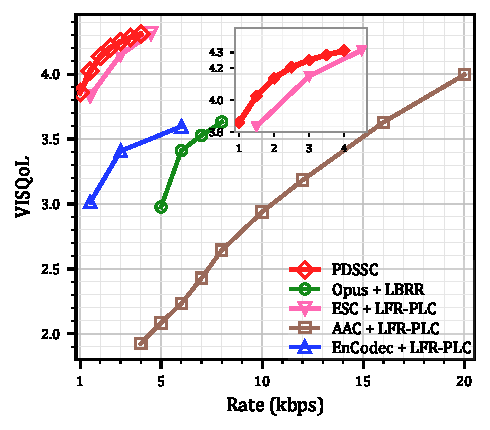
\includegraphics[width=0.85\linewidth]{paper_figs/fig4_visqol.pdf}\\[2mm]
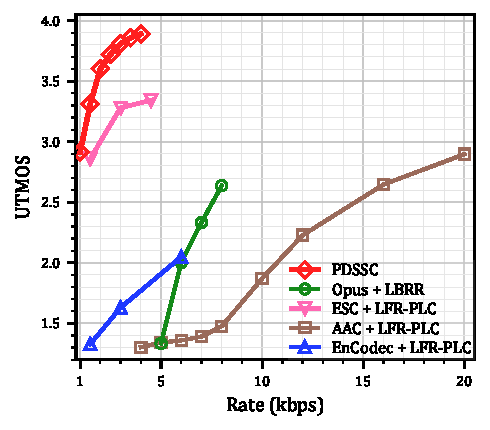
\includegraphics[width=0.85\linewidth]{paper_figs/fig4_utmos.pdf}
\caption{ViSQOL and UTMOS vs.\ bitrate under 5\% packet loss.}
\label{fig:rate}
\end{figure}

Relative to EnCodec, the advantage is even more revealing: both are discrete neural codecs, but PDSSC maintains a markedly better quality-bitrate tradeoff in the low-rate region. The gain therefore does not come merely from replacing a conventional codec with a neural one, but from reorganizing the transmitted information into a progressive semantic hierarchy and compensating the omitted residual detail at the receiver. ESC, the strongest existing low-bitrate baseline, also carries packet-loss protection and thus serves as a demanding comparison: at 1.0 kbps PDSSC already matches the perceptual quality that ESC attains only at 1.5 kbps (3.86 versus 3.83 in ViSQOL)---improving over such a protected baseline at a lower rate indicates a genuine gain in representation efficiency. As the insets show, a similar margin persists at neighboring operating points, where PDSSC surpasses ESC while using fewer bits.

To confirm that the quality-bitrate gain stems from the semantic ordering, Fig.~\ref{fig:disentangle} visualizes the layer-wise feature organization of PDSSC and EnCodec across three stages---the first quantization layer, the second layer, and the aggregation of layers 2--8---with each point coloured by speaker. In PDSSC, the first-layer points are uniformly spread with no visible speaker grouping, indicating that this layer has largely stripped speaker-dependent variation and kept a speaker-invariant semantic organization. At the second layer, which is distilled toward speaker timbre, the points of the same speaker begin to collapse into clusters while the inter-speaker separations widen. Summing layers 2--8 further tightens these clusters, as the remaining layers progressively fill in prosody, fine spectral detail, and other residual acoustic attributes that are largely speaker-dependent. This evolution, from dispersed points to compact intra-speaker clusters with large inter-speaker margins, is exactly what the two-level semantic-priority distillation should look like: the first layer carries the content shared across speakers, the second carries the speaker timbre, and the remaining layers absorb the residual prosodic and acoustic detail.

EnCodec behaves differently: its first-layer points already form diffuse, overlapping speaker clusters, so semantic content is never cleanly separated from speaker identity at the bottom of the hierarchy, and the clusters remain loosely organized with no clear progressive tightening in the higher stages. In other words, EnCodec's features stay coupled across layers, so lowering its bitrate prunes semantic and non-semantic information together rather than mainly trimming the refinable residual, whereas PDSSC's clear progressive separation ensures that bitrate reduction mainly suppresses the residual content while preserving the part most critical to intelligibility.


\begin{figure}[tb]
\centering
\makebox[\linewidth][c]{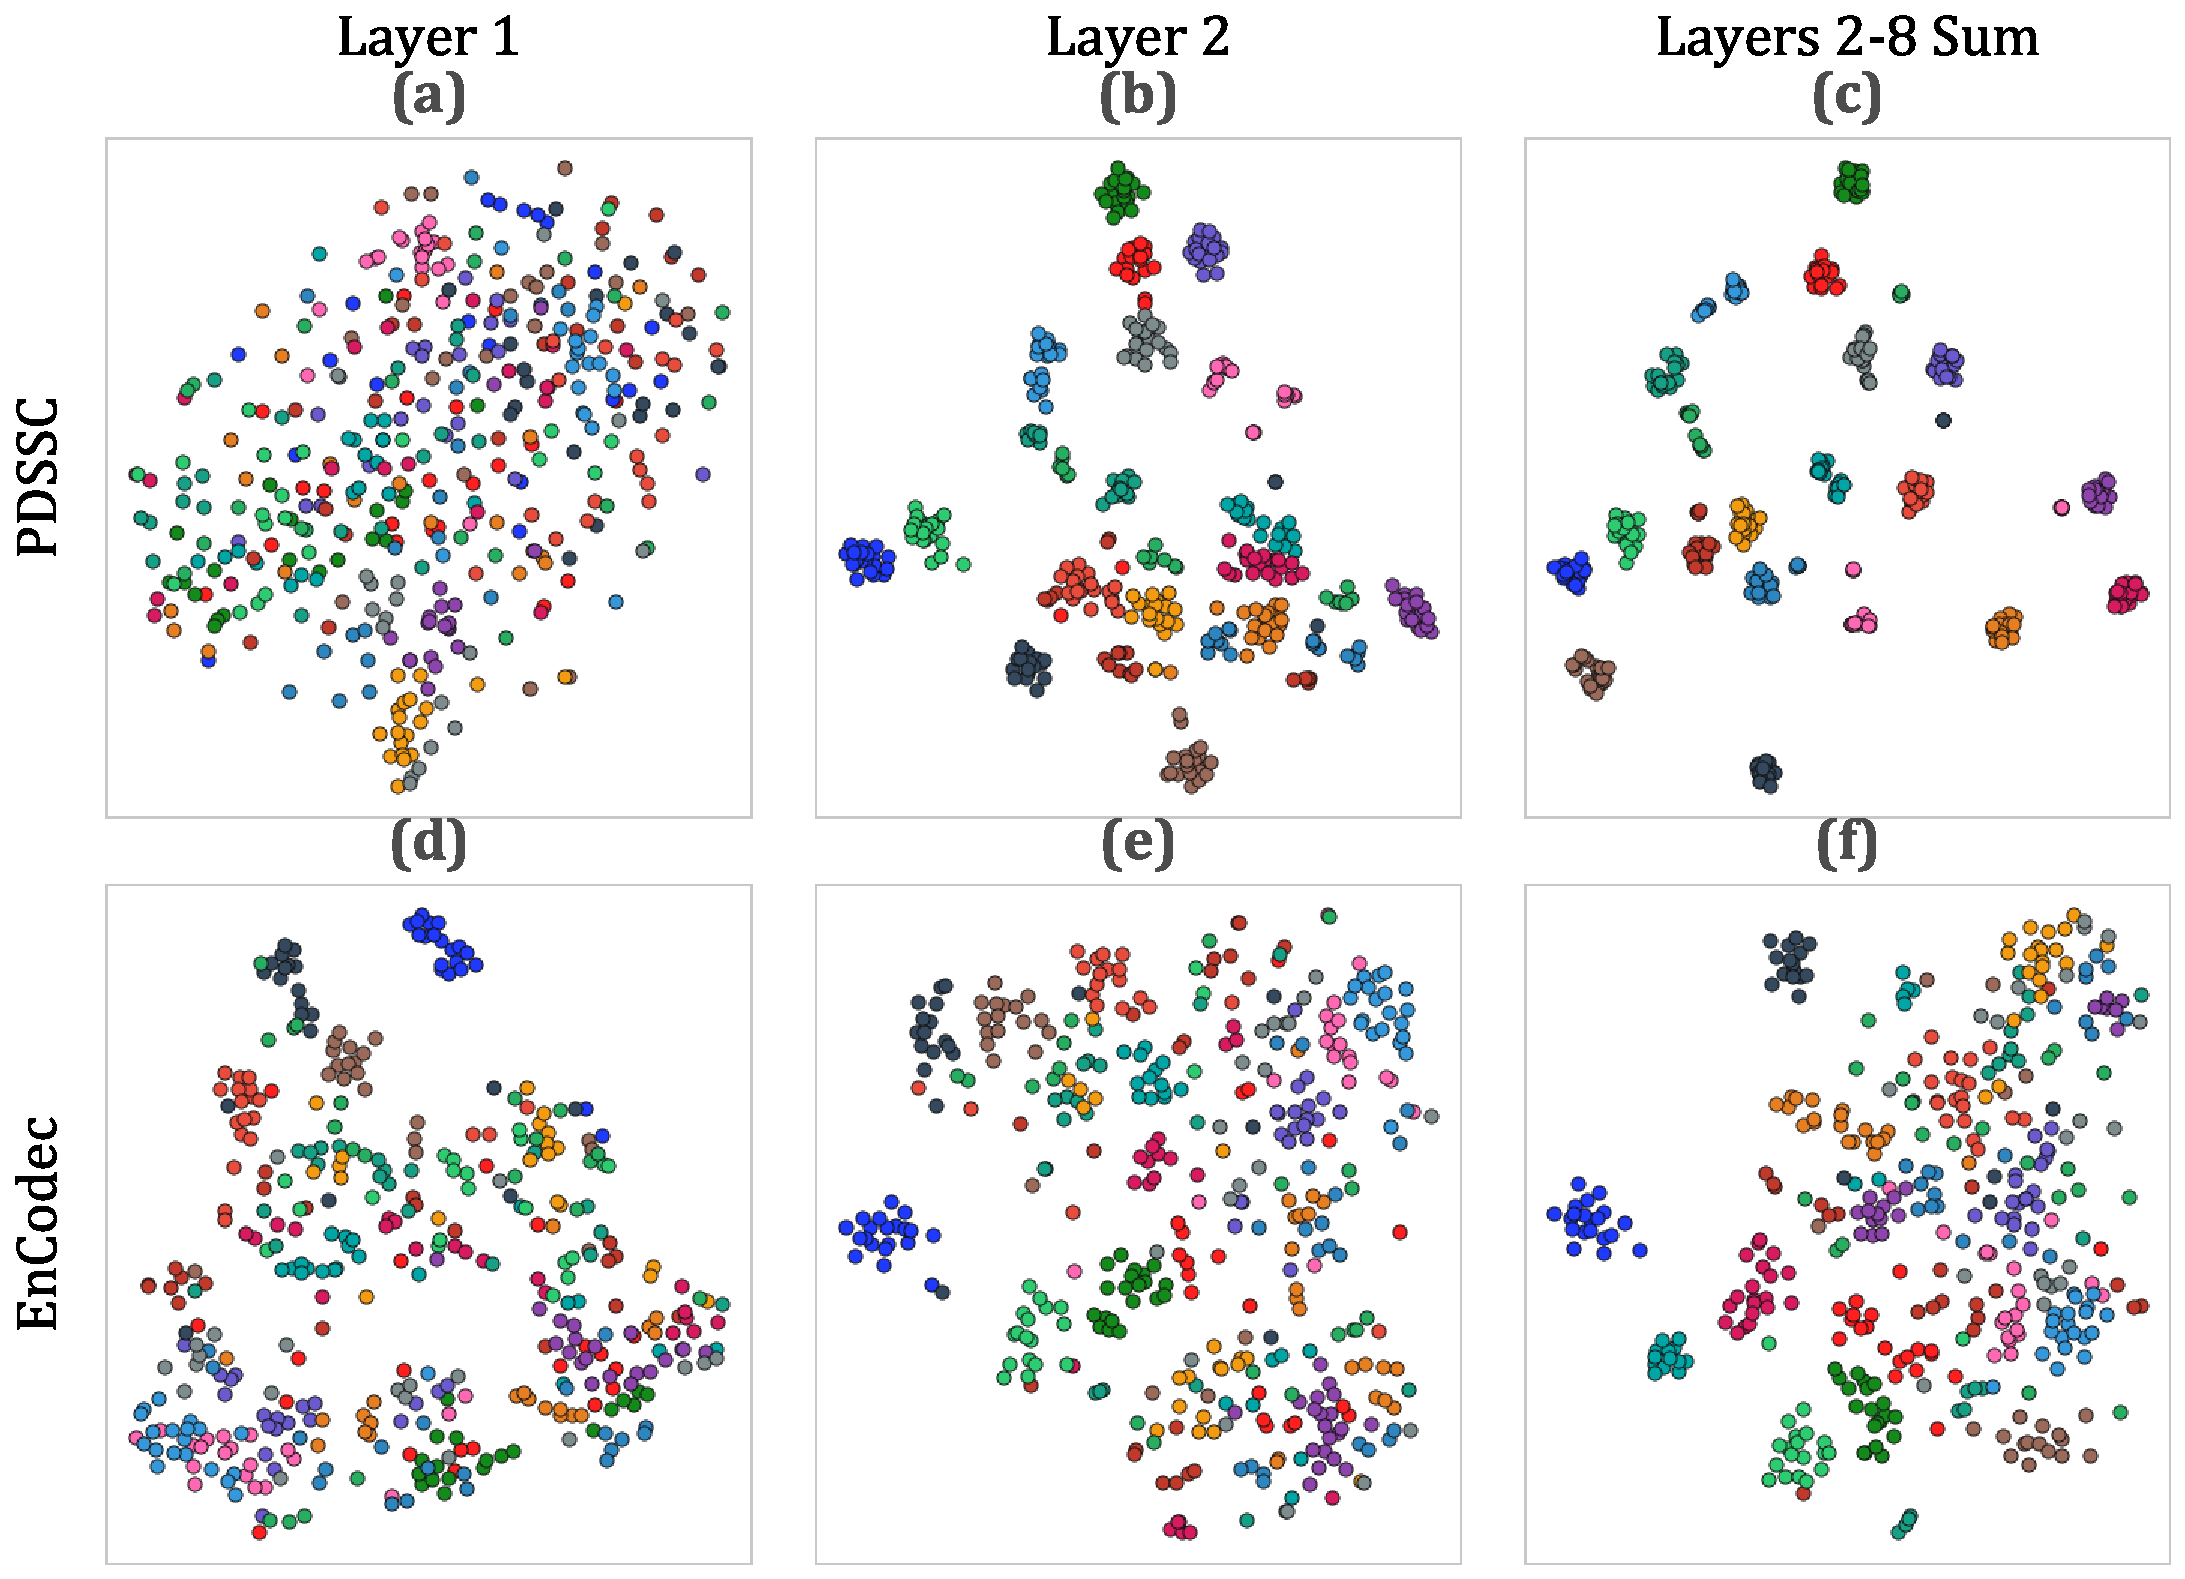
\includegraphics[width=1.0\linewidth]{paper_figs/fig5.pdf}}
\caption{Layer-wise feature visualization of PDSSC and EnCodec.}
\label{fig:disentangle}
\end{figure}

\subsection{Packet-Loss Robustness}

We next examine robustness under increasing packet loss, as shown in Fig.~\ref{fig:plr}. PDSSC is tested at average 1.5 and 3.0 kbps, while the competing methods run at their corresponding operating points, including higher-rate protected baselines such as Opus at 8.0 kbps; ViSQOL again measures overall speech quality, and PLCMOS~\cite{diener2023plcmos} serves as a non-intrusive perceptual metric designed for packet-loss concealment. PDSSC degrades much more gracefully than the competing methods as the channel becomes unreliable: under both bitrate reduction and packet erasure, the missing components are dominated by higher-layer speaker-related and other content-irrelevant residual attributes, while most of the semantic backbone is still preserved in the received latent representation. The recovery model is therefore highly targeted---it uses same-speaker prior knowledge to compensate for the missing high-layer detail on top of an already informative latent observation, so the restored quality remains stable even when channel losses become more severe.

\begin{figure}[tb]
\centering
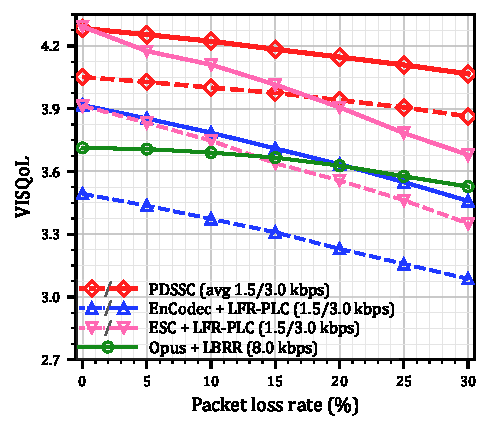
\includegraphics[width=0.85\linewidth]{paper_figs/fig6_visqol.pdf}\\[2mm]
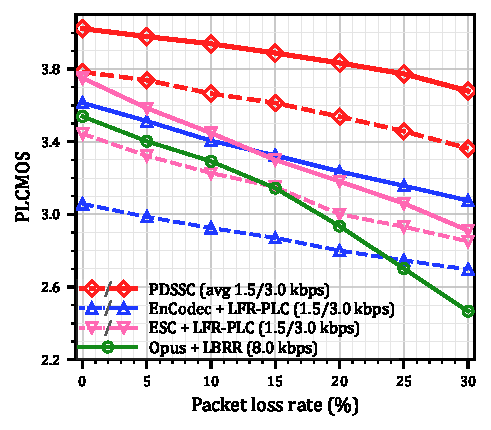
\includegraphics[width=0.85\linewidth]{paper_figs/fig6_plcmos.pdf}
\caption{ViSQOL and PLCMOS vs.\ packet loss rate.}
\label{fig:plr}
\end{figure}

On ViSQOL the margin holds at every loss point: at 3.0 kbps PDSSC stays above 4.0 across the entire loss range and above 3.8 at 1.5 kbps. The descent is markedly slower as well: PDSSC loses only about 0.2 over the full 0--30\% span, whereas ESC loses roughly three times as much and EnCodec twice as much. The slower decay is not merely cosmetic: because the baselines fall faster, the margins over them actually widen as the channel degrades, so the robustness advantage grows exactly when the channel is least reliable. The reason is structural: bitrate reduction and packet loss both strike predominantly the same component---the higher-layer residual---and most of that residual is speaker-related, since the second layer is distilled toward timbre and layers 2--8 carry prosody and other largely speaker-dependent detail. The recovery model therefore supplies exactly what is missing: the speaker reference embedding is available at the receiver at zero bandwidth cost and unaffected by channel distortion, so the regenerated detail matches the missing speaker characteristics, and the output loses finer detail rather than its foundation as the loss rate rises.

PLCMOS sharpens the contrast: being sensitive to concealment artifacts---inserted silence, repeated frames, and spectral mismatches---rather than to average quality, it rewards a system that genuinely regenerates the missing content and punishes one that merely fills the gap. This is exactly what separates PDSSC from the baselines: the missing high-layer detail---dominated by speaker-related factors---is regenerated in the latent domain by the generative recovery model from the semantic backbone and the speaker prior, so the restored frames stay acoustically consistent with their context and introduce no concealment artifacts. The baselines instead rely on redundancy or simple replacement, which erasure defeats: Opus with LBRR redundancy loses more than a full PLCMOS point over the range (3.54 to 2.47), since redundant frames are themselves erased under long bursts, and ESC loses 0.59 as its missing detail is left unrecovered. PDSSC instead descends only 0.34--0.42, retaining 3.68 in PLCMOS at 3.0 kbps even under 30\% loss. The contrast is therefore qualitative rather than a matter of degree: what decides the outcome is how the missing detail is repaired---regenerated in the latent domain from available side information, rather than redundantly retransmitted or crudely filled in---and PDSSC is the only system that repairs it in this way.

\subsection{Ablation Study}

We isolate the roles of the individual design components through the ablation results in Fig.~\ref{fig:abl}, which compares the full system at 1.5 kbps with three variants over the same packet-loss range, each disabling one component: the receiver-side recovery model, the semantic ordering, and the bitrate controller. Removing the recovery model first affects the system almost exclusively under loss: the ViSQOL margin of the full system over the no-recovery variant widens from 0.05 at 0\% loss to 0.19 at 30\% loss, and PLCMOS amplifies the difference from 0.43 to 0.72. Without recovery, quality collapses once the loss exceeds what the layered framework alone can absorb, ending at 2.63 in PLCMOS at 30\% loss and 1.5 kbps. The module's purpose is precisely to keep the recovered quality stable against channel loss: by regenerating the missing high-layer detail instead of leaving a hole in the latent, it sustains the output as erasures accumulate, so that quality decays gradually rather than dropping off a cliff.

Removing the semantic ordering, in contrast, hurts the quality level itself: it lowers ViSQOL by 0.26 at 0\% loss (4.05 versus 3.79) and PLCMOS by 0.78 at 0\% loss, widening to 0.89 at 30\% loss. The variant starts low but declines slowly, yet not as slowly as the full system (0.54 versus 0.43 in PLCMOS). This is because the ordering decides what the limited bits carry: with it, rate reduction trims residual detail that recovery can regenerate, so the decline stays moderate; without it, the cut can fall on the content that dominates quality, which recovery cannot restore. Even the no-recovery variant, which retains the ordering, finishes above the ordering-ablation one at 30\% loss (2.63 versus 2.46 in PLCMOS).

\begin{figure}[tb]
\centering
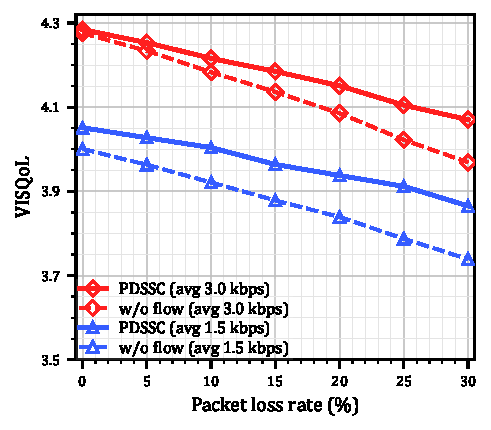
\includegraphics[width=0.85\linewidth]{paper_figs/fig8_visqol.pdf}\\[2mm]
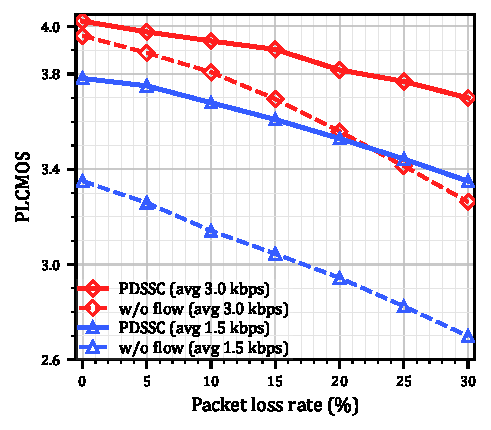
\includegraphics[width=0.85\linewidth]{paper_figs/fig8_plcmos.pdf}
\caption{Ablation of the individual design components.}
\label{fig:abl}
\end{figure}

Finally, without the controller, the system would transmit the same rate in every channel state, wasting bandwidth when the channel is good and sacrificing quality when it deteriorates. With the controller, the gear follows the channel automatically, and at equal average bitrate the quality is only marginally better than a fixed-gear policy---its value thus lies in the stability it provides under a time-varying channel rather than in peak quality. Moreover, it occupies negligible memory and computation (see Table~\ref{tab:complexity}), making it lightweight, easy to deploy, and efficient in operation.

\subsection{Qualitative Analysis and Deployment Efficiency}

We complement the quantitative results with a qualitative time-frequency view and an assessment of the computational and real-time cost of PDSSC. Fig.~\ref{fig:mel_compare} compares a representative mel-spectrogram from the test set. The spectrum reconstructed by PDSSC stays visibly closer to the original: harmonic stripes remain sharp and continuous across frames, and formant trajectories keep their natural bending rather than being flattened. The competing baselines, in contrast, exhibit more pronounced over-smoothing, local blurring around transient onsets, and missing fine detail in the upper spectral region, which together flatten perceptually salient cues---consistent with the quantitative gains above, and indicating that the advantage of PDSSC is a structural reconstruction improvement rather than a single-metric artifact. Whether this improvement is practical depends on its computational cost, examined next.

\begin{figure}[tb]
\centering
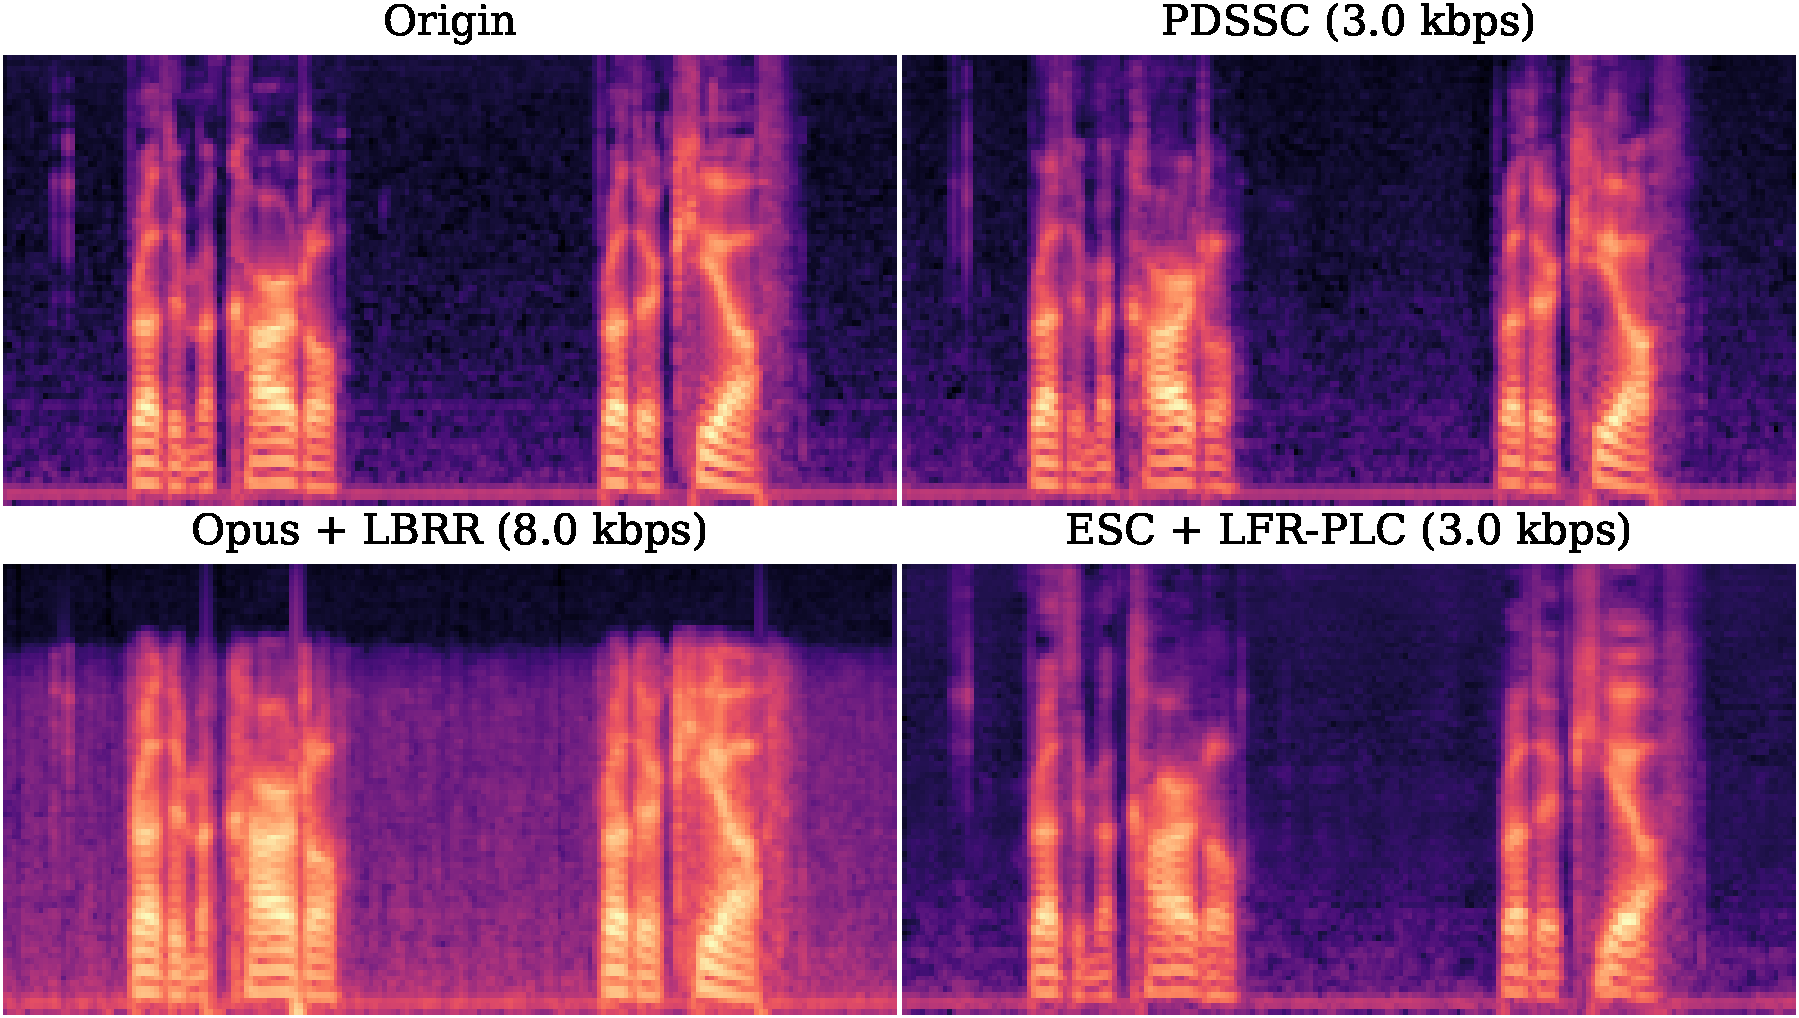
\includegraphics[width=1.0\linewidth]{paper_figs/fig7.pdf}
\caption{Mel-spectrogram comparison of PDSSC and competing methods.}
\label{fig:mel_compare}
\end{figure}

On the deployment side, Tables~\ref{tab:complexity} and~\ref{tab:latency} report the computational and real-time cost of PDSSC. Table~\ref{tab:complexity} shows that cost is concentrated where it is unavoidable---the semantic encoder and decoder---while the modules that differentiate PDSSC remain light: the RVQ codebooks add moderate complexity, the adaptive controller is essentially negligible, and the generative recovery model is markedly lighter than the backbone itself. This distribution is deliberate: the robustness gain comes from a targeted, low-step recovery mechanism rather than an over-parameterized receiver, so the distinguishing quality and robustness do not translate into proportional deployment cost.

\begin{table}[tb]
\caption{Model complexity of the proposed PDSSC system.}
\label{tab:complexity}
\centering
\footnotesize
\renewcommand{\arraystretch}{0.92}
\begin{tabular}{lcc}
\hline
Module & GFLOPs & Params (M) \\
\hline
Semantic Encoder & 58.694 & 103.676 \\
RVQ Codebooks & 4.198 & 8.389 \\
Adaptive Controller & 0.008 & 0.031 \\
Generative Recovery Model & 11.726 & 58.470 \\
Semantic Decoder & 111.256 & 103.676 \\
Total & 185.882 & 274.242 \\
\hline
\end{tabular}
\end{table}

The latency comparison in Table~\ref{tab:latency} corroborates this observation. At a common 3.0~kbps operating point, PDSSC attains an average model latency of 0.151~s, well below the 400-ms one-way delay budget for interactive speech~\cite{itu_t_g114} and substantially lower than the semantic baselines ESC (0.330~s) and LargeSC~\cite{tian2025lsm} (0.460~s), owing to the low-step recovery design requiring fewer iterative denoising steps and a shorter buffering window. EnCodec and Opus~+~LBRR are faster still (0.103~s and 0.071~s), but they only have speed: EnCodec at the same 3.0~kbps rate falls short in quality and packet-loss robustness, as reported above, and Opus~+~LBRR needs 8.0~kbps, beyond the low-bitrate budget. Neither reaches the performance and bitrate requirements of the target scenario, whereas PDSSC---at 0.151~s, well within the 400-ms interactive budget---meets all three.

\begin{table}[tb]
\caption{End-to-end latency comparison of PDSSC and competing methods.}
\label{tab:latency}
\centering
\footnotesize
\renewcommand{\arraystretch}{0.92}
\begin{tabular}{lccc}
\hline
Method & Sample rate (kHz) & Bitrate (bps) & Delay (s) \\
\hline
PDSSC & 16.0 & 3000 & 0.151 \\
EnCodec + LFR-PLC & 24.0 & 3000 & 0.103 \\
ESC + LFR-PLC & 16.0 & 3000 & 0.330 \\
LargeSC & 24.0 & 2060 & 0.460 \\
Opus + LBRR & 24.0 & 8000 & 0.071 \\
\hline
\end{tabular}
\end{table}

\section{Conclusion}
In this paper, we proposed PDSSC, which combines a semantic-priority layered discrete representation, speaker-guided low-step generative recovery, and lightweight bitrate control for progressive digital semantic speech communication over low-bitrate, packet-loss-prone channels. Experimental results show that it attains a ViSQOL of 4.14 at 2.0~kbps---exceeding Opus at 8.0~kbps---and retains 3.68 in PLCMOS at 3.0~kbps even under 30\% packet loss, degrading far more gracefully than the compared baselines while remaining practical for real-time deployment. Future work includes lower-latency streaming recovery and evaluation under more realistic wireless conditions.

\begin{thebibliography}{00}
\setlength{\itemsep}{0pt}
\setlength{\parsep}{0pt}

\bibitem{3gpp_ntn} 3GPP, ``Non-terrestrial networks (NTN),'' accessed May 12, 2026. [Online]. Available: \url{https://www.3gpp.org/technologies/ntn-overview}

\bibitem{cui2022sagin} H. Cui, J. Zhang, Y. Geng, Z. Xiao, T. Sun, N. Zhang, J. Liu, Q. Wu, and X. Cao, ``Space-air-ground integrated network (SAGIN) for 6G: Requirements, architecture and challenges,'' \emph{China Communications}, vol. 19, no. 2, pp. 90--108, Feb. 2022.

\bibitem{ngmn_ntn} NGMN Alliance, ``Non-terrestrial networks position paper,'' Dec. 2019. [Online]. Available: \url{https://www.ngmn.org/wp-content/uploads/Publications/2019/191209-NGMN-Non-Terrestrial-Networks-Position-Paper.pdf}

\bibitem{iso_aac} ISO/IEC, ``Information technology -- Coding of audio-visual objects -- Part 3: Audio,'' ISO/IEC 14496-3:2019, 2019.

\bibitem{valin2012opus} J.-M. Valin, K. Vos, and T. Terriberry, ``Definition of the Opus audio codec,'' IETF RFC 6716, Sept. 2012.

\bibitem{qin2021semcom} Z. Qin, X. Tao, J. Lu, W. Tong, and G. Y. Li, ``Semantic communications: Principles and challenges,'' arXiv preprint arXiv:2201.01389, 2021. [Online]. Available: \url{https://arxiv.org/abs/2201.01389}

\bibitem{nguyen2025survey} L. X. Nguyen, A. D. Raha, P. S. Aung, D. Niyato, Z. Han, and C. S. Hong, ``A contemporary survey on semantic communications: Theory of mind, generative AI, and deep joint source-channel coding,'' arXiv preprint arXiv:2502.16468, 2025. [Online]. Available: \url{https://arxiv.org/abs/2502.16468}

\bibitem{weng2020deepscs} Z. Weng, Z. Qin, and G. Y. Li, ``Semantic communications for speech signals,'' arXiv preprint arXiv:2012.05369, 2020. [Online]. Available: \url{https://arxiv.org/abs/2012.05369}

\bibitem{xie2021deepsc} H. Xie, Z. Qin, G. Y. Li, and B.-H. Juang, ``Deep learning enabled semantic communication systems,'' \emph{IEEE Transactions on Signal Processing}, vol. 69, pp. 2663--2675, 2021.

\bibitem{weng2022deepscst} Z. Weng, Z. Qin, X. Tao, C. Pan, G. Liu, and G. Y. Li, ``Deep learning enabled semantic communications with speech recognition and synthesis,'' arXiv preprint arXiv:2205.04603, 2022. [Online]. Available: \url{https://arxiv.org/abs/2205.04603}

\bibitem{xiao2023dsst} Z. Xiao, S. Yao, J. Dai, S. Wang, K. Niu, and P. Zhang, ``Wireless deep speech semantic transmission,'' in \emph{Proc. IEEE International Conference on Acoustics, Speech and Signal Processing (ICASSP)}, 2023.

\bibitem{defossez2023encodec} A. D\'efossez, J. Copet, G. Synnaeve, and Y. Adi, ``High fidelity neural audio compression,'' \emph{Transactions on Machine Learning Research}, 2023.

\bibitem{kumar2023dac} R. Kumar, P. Seetharaman, S. Luebs, A. Kumar, and K. Kumar, ``High-fidelity audio compression with improved RVQGAN,'' in \emph{Proc. Advances in Neural Information Processing Systems (NeurIPS)}, 2023.

\bibitem{chen2025rvqgan} X. Chen, J. Wang, J. Huang, M. Zeng, Z. Zheng, and Z. Fei, ``Low-bitrate high-quality digital semantic communication based on RVQGAN,'' \emph{IEEE Internet of Things Journal}, vol. 12, no. 10, pp. 13525--13537, 2025.

\bibitem{xin2024bigcodec} D. Xin, X. Tan, S. Takamichi, and H. Saruwatari, ``BigCodec: Pushing the limits of low-bitrate neural speech codec,'' arXiv preprint arXiv:2409.05377, 2024. [Online]. Available: \url{https://arxiv.org/abs/2409.05377}

\bibitem{gu2024esc} Y. Gu and E. Diao, ``ESC: Efficient speech coding with cross-scale residual vector quantized transformers,'' in \emph{Proc. Conference on Empirical Methods in Natural Language Processing (EMNLP)}, 2024, pp. 10084--10096.

\bibitem{rodriguez2024diffusion} E. Grassucci, C. Marinoni, A. Rodriguez, and D. Comminiello, ``Diffusion models for audio semantic communication,'' in \emph{Proc. IEEE International Conference on Acoustics, Speech and Signal Processing (ICASSP)}, 2024, pp. 13136--13140.

\bibitem{tian2025lsm} Y. Tian, Z. Qin, G. Lv, Y. Jin, K. Huang, and Z. Han, ``Large speech model enabled semantic communication,'' arXiv preprint arXiv:2512.04711, 2025. [Online]. Available: \url{https://arxiv.org/abs/2512.04711}

\bibitem{han2025esc} Z. Han, J. Dai, S. Yao, J. Wang, Y. Li, K. Niu, W. Xu, and P. Zhang, ``Error-resilient semantic communication for speech transmission over packet-loss networks,'' arXiv preprint arXiv:2512.08203, 2025. [Online]. Available: \url{https://arxiv.org/abs/2512.08203}

\bibitem{gilbert1960} E. N. Gilbert, ``Capacity of a burst-noise channel,'' \emph{Bell System Technical Journal}, vol. 39, no. 5, pp. 1253--1265, Sep. 1960.

\bibitem{elliott1963} E. O. Elliott, ``Estimates of error rates for codes on burst-noise channels,'' \emph{Bell System Technical Journal}, vol. 42, no. 5, pp. 1977--1997, Sep. 1963.

\bibitem{oord2017vqvae} A. van den Oord, O. Vinyals, and K. Kavukcuoglu, ``Neural discrete representation learning,'' in \emph{Proc. Advances in Neural Information Processing Systems (NeurIPS)}, 2017.

\bibitem{hsu2021hubert} W.-N. Hsu, B. Bolte, Y.-H. H. Tsai, K. Lakhotia, R. Salakhutdinov, and A. Mohamed, ``HuBERT: Self-supervised speech representation learning by masked prediction of hidden units,'' \emph{IEEE/ACM Transactions on Audio, Speech, and Language Processing}, vol. 29, pp. 3451--3460, 2021.

\bibitem{desplanques2020ecapa} B. Desplanques, J. Thienpondt, and K. Demuynck, ``ECAPA-TDNN: Emphasized channel attention, propagation and aggregation in TDNN-based speaker verification,'' in \emph{Proc. Interspeech}, 2020, pp. 3830--3834.


\bibitem{lipman2023flow} Y. Lipman, R. T. Q. Chen, H. Ben-Hamu, M. Nickel, and M. Le, ``Flow matching for generative modeling,'' in \emph{Proc. International Conference on Learning Representations (ICLR)}, 2023.

\bibitem{chen2022wavlm} S. Chen et al., ``WavLM: Large-scale self-supervised pre-training for full stack speech processing,'' \emph{IEEE/ACM Transactions on Audio, Speech, and Language Processing}, vol. 30, pp. 3388--3402, 2022.

\bibitem{panayotov2015librispeech} V. Panayotov, G. Chen, D. Povey, and S. Khudanpur, ``LibriSpeech: An ASR corpus based on public domain audio books,'' in \emph{Proc. IEEE International Conference on Acoustics, Speech and Signal Processing (ICASSP)}, 2015, pp. 5206--5210.

\bibitem{chinen2020visqolv3} M. Chinen, F. S. C. Lim, J. Skoglund, N. Gureev, F. O'Gorman, and A. Hines, ``ViSQOL v3: An open source production ready objective speech and audio metric,'' arXiv preprint arXiv:2004.09584, 2020. [Online]. Available: \url{https://arxiv.org/abs/2004.09584}

\bibitem{saeki2022utmos} T. Saeki, D. Xin, W. Nakata, T. Koriyama, S. Takamichi, and H. Saruwatari, ``UTMOS: UTokyo-SaruLab system for VoiceMOS Challenge 2022,'' in \emph{Proc. Interspeech}, 2022.

\bibitem{diener2023plcmos} L. Diener, M. Purin, S. Sootla, A. Saabas, R. Aichner, and R. Cutler, ``PLCMOS -- A data-driven non-intrusive metric for the evaluation of packet loss concealment algorithms,'' in \emph{Proc. Interspeech}, 2023, pp. 2533--2537.

\bibitem{itu_t_g114} ITU-T Recommendation G.114, ``One-way transmission time,'' International Telecommunication Union, 2003.

\end{thebibliography}

\end{document}
